%PART_3_CHAP_3
\myChapter{R}{ésultats quantitatifs}
%WAIT a Review ok
\begin{resumChap}[.92]
\setstretch{1,12}
C'est dans ce troisième et dernier chapitre de la partie 3 que nous aborderons les différentes expérimentations réalisées, avortées, ou en construction.
Il se divise en 4 grandes thématiques: \Li l'utilisabilité et l'expérience utilisateur offerte par le kit ErgoJr, \ii l'impact de ce kit sur l'acceptabilité globale de la robotique, \iii la motivation à effectuer des activités impliquant des robots et \iiii les connaissances et apprentissages réalisés lors de telles activités.\par%
Les deux premières concernent une étude réalisée sur une population ayant manipulé les robots en classe durant toute l'année.
Pour cette étude, le matériel de recherche s'est constitué principalement des questionnaires \sht{SUS} et \sht{ATT} pour la 1\iere thématique et des questionnaires \sht{EURO382} et \sht{NARS} pour la deuxième. Dans chacune de ces parties, est également présentée une expérimentation ponctuelle ayant complété les analyses déjà réalisées, soit en abordant différents contextes, soit en cherchant à comprendre certains mécanismes implicites (\ie le fait de donner un nom à son robot).\par%
Les deux thématiques abordées en suivant présentent uniquement des expérimentations ponctuelles. 
Concernant la motivation, une 1\iere étude\break \tiret{n'ayant pas abouti} sera évoquée, notamment au travers des ressources qui ont été développées initialement pour celle-ci. Une 2\ieme étude, sur l'impact de la contrôlabilité lors du montage d'un robot (un Poppy Dragtser) fut réalisée.
Une 3\ieme étude portant sur l'impact de certaines formulations dans la perception subjective de l'élève, fut également entreprise.
Concernant les apprentissages, dans cette même étude, un pan fut consacré à cette thématique, au travers d'un mini quiz. Une 2\nde étude sur cette thématique a été développée, notamment via la réalisation d'une étude pilote et la construction d'une étude contrôlée en découlant. Cependant, cette dernière n'a pas encore été réalisée.\par%
%Chacune de ces thématiques offrira une introduction et une synthèse.
\end{resumChap}{}
\begin{comment}
\begin{table}
    \centering
    \begin{tabular}{|c|l|c|c|c|}
        \hline
         \textbf{Page}&\textbf{Nom} & \textbf{Étude} & \textbf{Étude} & \textbf{Soumis,} \\
          & & \textbf{Pilote} & \textbf{Réel} & \textbf{ou Publié} \\\hline\hline
         \pageref{Exp:L_UX}&            Longitudinale utilisabilité \& \sht{UX}    & X & X & X \\\hline
         \pageref{Exp:euro}&            Longitudinale acceptabilité                     & X & X & - \\\hline
         \pageref{Exp:vs_thymio}&       Utilisabilité comparative                       & X & X & X \\\hline
         \pageref{Exp:name_for_bot}&    Un nom pour un robot                            & X & X & - \\\hline
         %\pageref{Exp:a_priorie}&       Les a-priorie en robotique                      & - & - & - \\\hline
         \pageref{Exp:Role_support}&    Rôle du support                                 & X & - & - \\\hline
         \pageref{Exp:dragster}&        Notice modulaire ou linéaire                    & X & X & - \\\hline
         \pageref{Exp:poule}&           Décrire ou manipuler                            & X & X & - \\\hline
         \pageref{Exp:Reel_virtuel}&    Robot réel ou virtuel                           & X & - & - \\\hline
    \end{tabular}
    \caption{Listes des expérimentations présentées}
    \label{tab:list_exp}
\end{table}\par%
\end{comment}
\subchapFont
%PART_3_CHAP_3_SEC_1
%WAIT a Review, ok
\section{Utilisabilité et UX}\label{Exp:L_UX}
    \subsection{Introduction}
        Pour réaliser cette étude, nous avons sélectionné deux questionnaires standardisés traitant de cette question: le \sht{SUS}~\citeA{pdf:SUS} et l' \sht{ATT}~\citeA{pdf:ATT}.
        Ces deux questionnaires sont complémentaires et permettent, d'un côté d'identifier d'éventuels problèmes de conception et de l'autre de rendre compte de la perception de l'utilisateur lors des activités.
        L’intérêt qu'ils soient standardisés est de pouvoir comparer les résultats.
    \paragraph{Méthode} 
        Le lien de ces questionnaires (à compléter en ligne) a été diffusé aux enseignants participant au dispositif Poppy-Éducation, qui l'ont ensuite transmis à leurs élèves.
        Nous avons collecté $88$ réponses: $20$ enseignants de $47$ ans en moyenne (écart type~$S=14,26$) et $68$ élèves ($\hat{a}ge=16$;~$S=2,44$),  $37$ sont issus de section ISN, $12$ de ICN, et $18$ du collège ($17$ de 3ème et $1$ de 4ème).
        Il ont tous pratiqué des activités durant l'année scolaire 2016 -- 2017 et ont répondu aux questionnaires à la fin de cette même année.
        Ces activités ont pu être plus ou moins longues, plus ou moins répétées;
        pour déterminer ces paramètres un questionnaire de renseignements additionnels était intégré après les questionnaires d'utilisabilité, permettant de dégager 29~critères de discrimination visibles sur la figure~\ref{fig:sus_val_moy} en page~\pageref{fig:sus_val_moy}.
        Nous avons également synthétisé certains de ces critères pour former des groupes:
        \textit{néophyte}, n'a pas utilisé d'autres kits et a pratiqué moins de 6~heures d'activités avec le kit ErgoJr;
        \textit{novice}, n'a pas utilisé d'autres kits et a pratiqué entre 6 et 25~heures d'activités avec le kit ErgoJr;
        \textit{expert}, a utilisé d'autres kits et a pratiqué plus de 25~heures d'activités avec le kit ErgoJr;
        cependant, ces groupes n'ont pas permis d'établir de distinction significative.
        En revanche, d'autres résultats peuvent être observés, en voici les principaux.
    \subsection{SUS}
        Nous pouvons observer sur la figure~\ref{fig:sus_chemin} que la moyenne générale (axe noir en gras) est positive sur l'ensemble des affirmations hormis la première, cela est peut-être induit par l'environnement scolaire proposant des plannings stricts et de nombreux modules à explorer.
        Les affirmations 4 et 8 offrent la plus grande variabilité suivant les modalités, l'affirmation 8 s'étale du \cro{non} à \cro{absolument non} montrant une bonne acceptance.
        L'affirmation 4 allant de \cro{non} à \cro{sans avis} associée aux affirmations 7, 3 et 10 (variant légèrement moins), évoquent les questions de prise en main et de capacité d'auto-formation, point que nous souhaitions optimiser.
        Ici cette variabilité semble montrer que notre action a eu un impact mais pas sur l'ensemble de la population.
        \begin{figure}[!h]
            \centering
            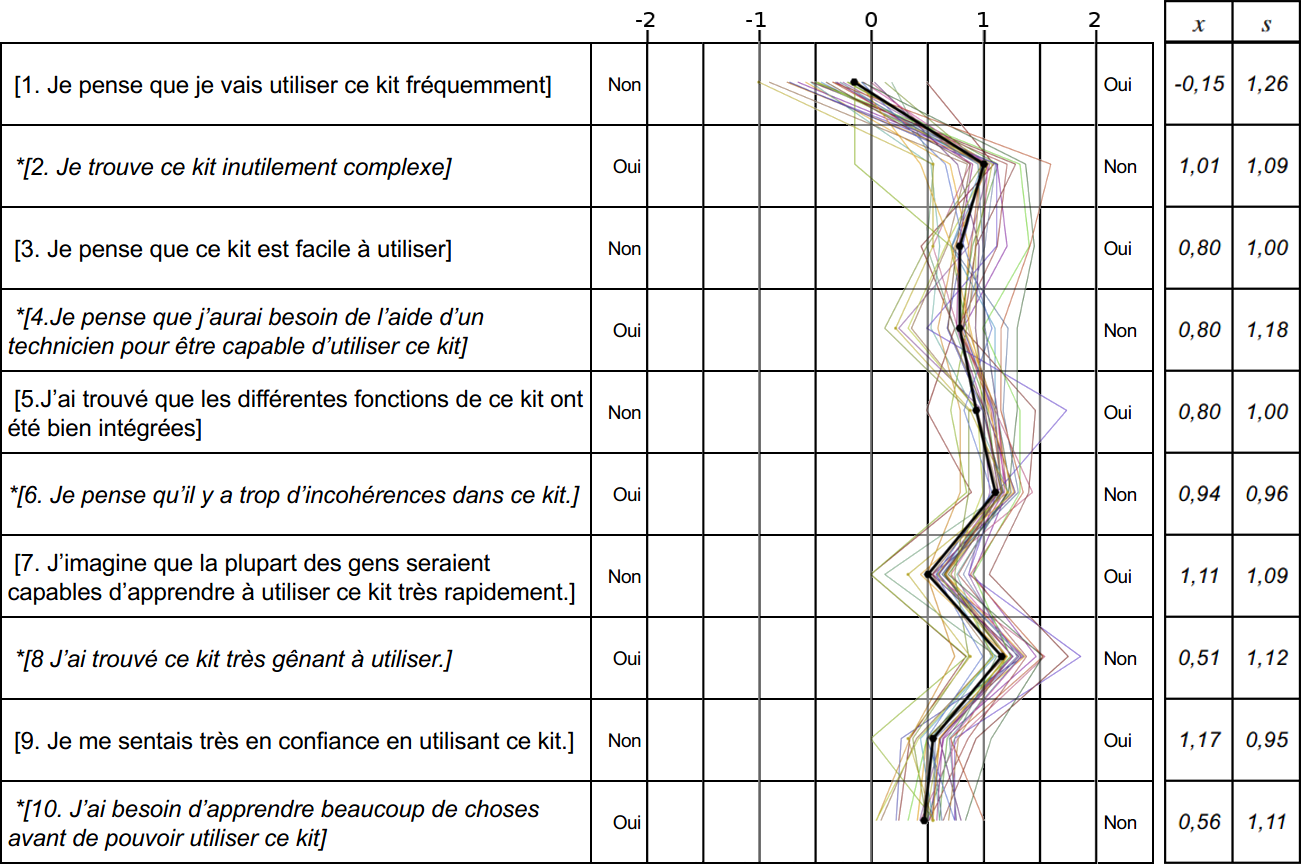
\includegraphics[width=0.9\linewidth]{Figures/Desprez_didapro-sus_chemin.png}
            \caption{Résultats SUS~\citeB{desprez2018poppy}}\label{fig:sus_chemin}
        \end{figure}
        La rétrospective de 2013 du \sht{SUS}~\citeB{brooke2013sus} nous apprend que le score moyen obtenu par des dispositifs au \sht{SUS} est de $68/100$ soit $0,72$ sur l'intervalle $[-2;2]$.
        Dans notre étude, la moyenne générale a atteint $0,72$: $0,57$ pour les enseignants et $0,77$ pour les élèves.
        Lorsque nous observons les résultats avec plus de détails, nous pouvons nous apercevoir (\textit{cf} Figure~\ref{fig:sus_val_moy}) que certains usages font varier significativement le score du \sht{SUS} de la moyenne ($Test\ de\ Student\ bilat\acute{e}ral\;\ \alpha=0,05\;\ ddl=9\;\ variable\ de\ r\acute{e}f\acute{e}rence=modalit\acute{e}\ \acute{E}l\grave{e}ves$), notamment:
        un temps d'utilisation inférieur à 2~heures ($p=0,0238$) ou une longue période entre la dernière utilisation du kit et le passage du questionnaire ($p=0,0007$) qui l'impacte négativement;
        l'utilisation du livret pédagogique ($p=0,0004$) qui l'impacte positivement;
        le choix du langage de programmation (\sht{snap} $p=0,0017$; python $p=0,0103$; autre $p=0,0019$) ayant un impact relatif au choix effectué:
        positif pour \sht{snap}, négatif pour python ou les autres langages (non natifs).\par%
        D'autre part, il est également intéressant d'observer les critères ne faisant pas varier significativement le score du \sht{SUS} comme l'utilisation d'autres kits ($p=0,3357$) ou non ($p=0,1683$);
        la construction du robot ($p=0,1029$) ou non ($p=0,2996$);
        ou encore la distinction entre \textit{Enseignants/Élèves} ($p=0,1687$) qui étaient des critères attendus comme discriminants.
        Cependant, concernant cette dernière, le faible effectif côté enseignants ($N=20$) peut expliquer l'absence de différence significative (\textit{cf 4.Limites \& perspectives}).
        Enfin, nous n'observons pas de distinction \textit{Homme/Femme} ($p=0,3740$), comme il est courant de trouver dans d'autres disciplines.
        \begin{figure}[!h]
            \centering
            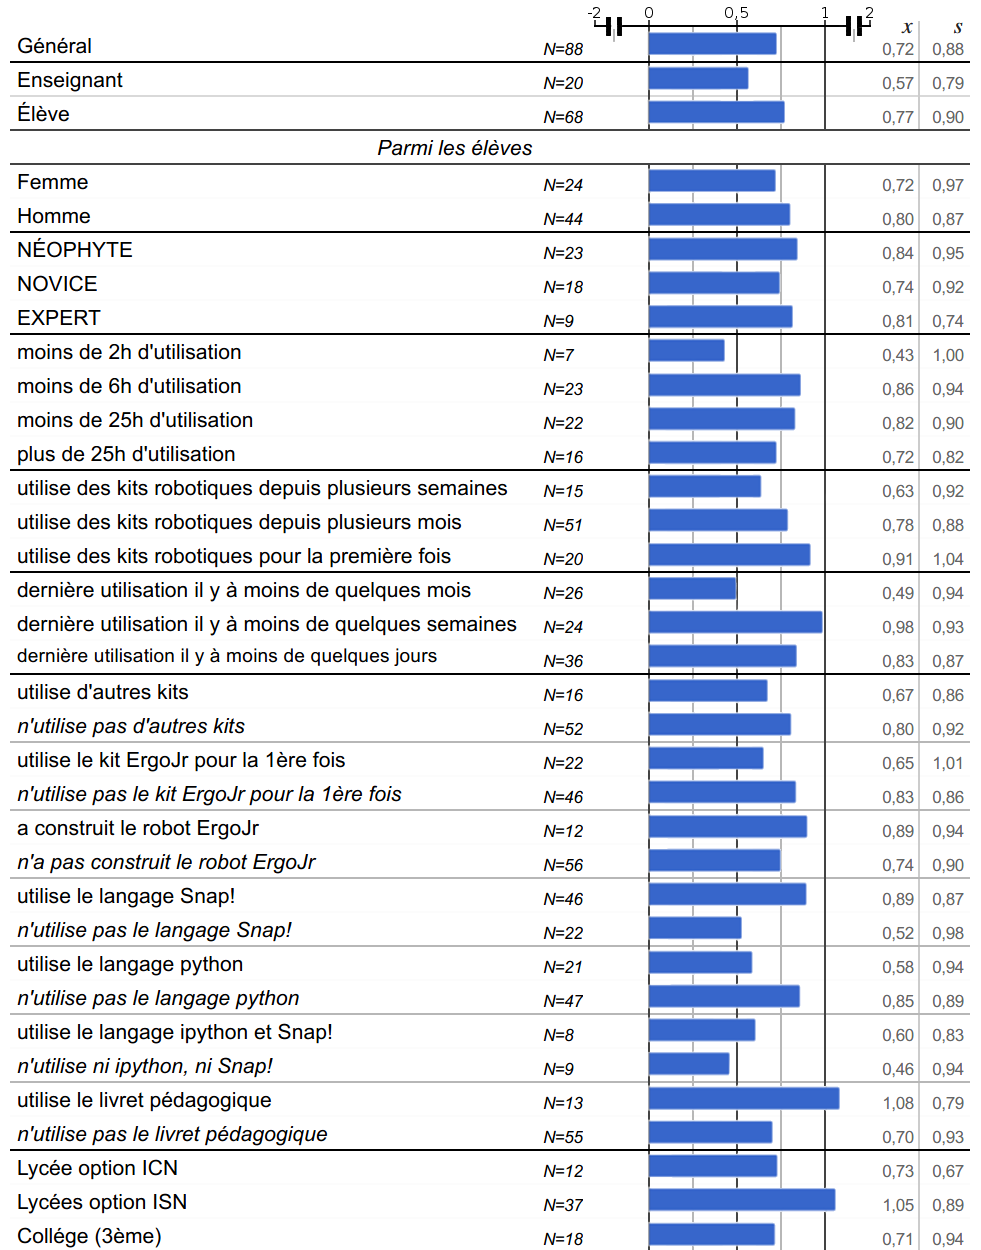
\includegraphics[width=0.9\linewidth]{Figures/Desprez_didapro-sus_val_moy.png}
            \caption{Résultats SUS, valeurs par groupes}\label{fig:sus_val_moy}
        \end{figure}
    \subsection{AttrackDiff}
        Nous pouvons observer sur la figure~\ref{fig:attrakdiff_chemin} le résultat pour nos 29 modalités pour les 28 paires de mots, ici ordonnées par catégorie.
        Sur la figure~\ref{fig:attrakdiff_chemin} nous pouvons voir qu'une majorité de réponses sont positives, et que plusieurs paires de mots semblent se distinguer, notamment:
        l'évaluation de \textit{Technique~/~Humain} en moyenne à $\overline{x}=-0,70$~($S= 1,38$) et l'évaluation de \textit{Amateur~/~Professionnel} à $\overline{x}=-0,15$~($S=1,45$) quand l'évaluation générale se situe à $\overline{x}=1,20$~($S=0,61$).
        Dans une moindre mesure nous observons la même distinction au niveau de \textit{Prévisible~/~Imprévisible} $\overline{x}=0,36$~($S=1,31$) qui peut s'expliquer par la mise en avant dans les activités de la démarche d'apprentissage par essai-erreur.
        De la même façon on observe que les termes \textit{Original - Créatif - Plaisant} obtiennent une meilleure évaluation que la moyenne, respectivement: $\overline{x}= 1,73; 1,75; 1,88$~($S= 1,24; 1,14; 1,15$).
        \begin{figure}[!h]
            \centering
            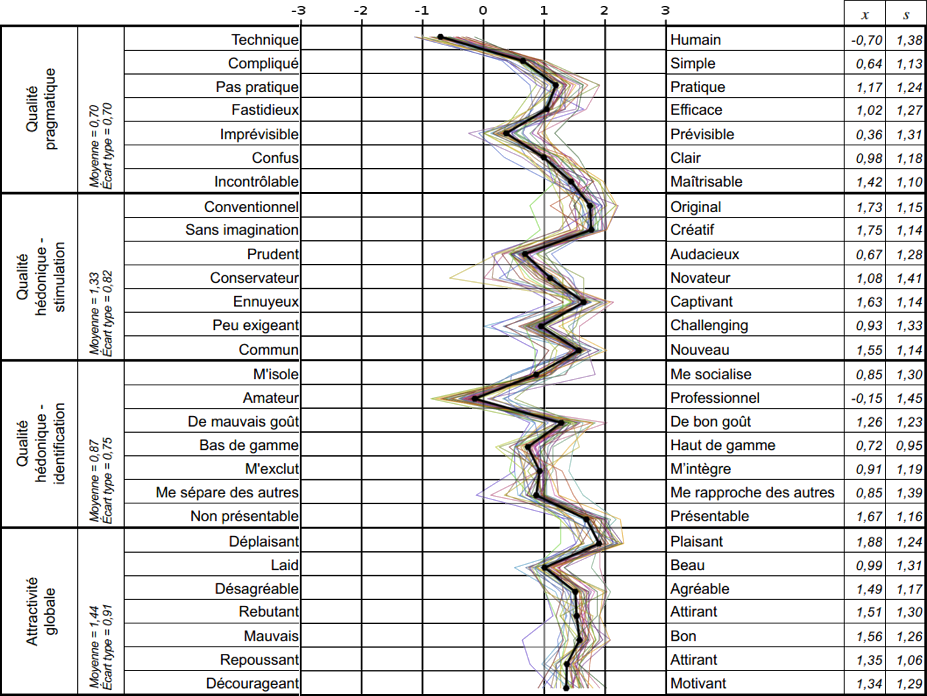
\includegraphics[width=0.9\linewidth]{Figures/Desprez_didapro-attrakdiff_chemin.png}
            \caption{Résultats \textit{AttrakDiff}~\citeB{desprez2018poppy}}\label{fig:attrakdiff_chemin}
        \end{figure}\par%
        Au niveau des 4 échelles, nous observons que l'aspect stimulation $\overline{x}=1,33$~($S=0,70$) et l'attractivité globale $\overline{x}=1,44$~($S=0,91$) obtiennent de meilleurs résultats que l'aspect identification $\overline{x}=0,87$~($S=0,75$) et pragmatique $\overline{x}=0,70$~($S=0,70$).
        La moyenne de ces différentes échelles donne un score global de $1,087$~($S=0,58$) pour l'ensemble de l'échantillon ($N=88$); de $1,057$~($S=0,58$) pour les enseignants ($N=20$); et de $1,182$~($S=0,61$) pour les élèves ($N=68$).
        Mais une représentation à deux dimensions nous permettra d'appréhender les résultats de manière plus efficiente.
        Ainsi nous pouvons observer, notamment sur la figure~\ref{fig:attrakdiff_point}, que la répartition globale est plutôt bien localisée:
        la moyenne générale se situe à $\overline{x}=1,07$~($S=0,64$) qui correspond à la valeur moyenne obtenue aux échelles \gui{Qualité~Pragmatique} et \gui{Attractivité~Globale}; et $\overline{y}=1,09$~($S=0,53$) qui correspond à la valeur moyenne obtenue aux échelles \gui{Qualité~Hédonique~Stimulation} et \gui{Identité}.
        En regardant par le prisme de nos 29 modalités, Nous observons que le nuage de points est plutôt homogène, mais certaines modalités (présentées sur la figure~\ref{fig:attrakdiff_point}) obtiennent des valeurs plus extrêmes par rapport à notre échantillon de base.
        \begin{figure}[!h]
            \centering
            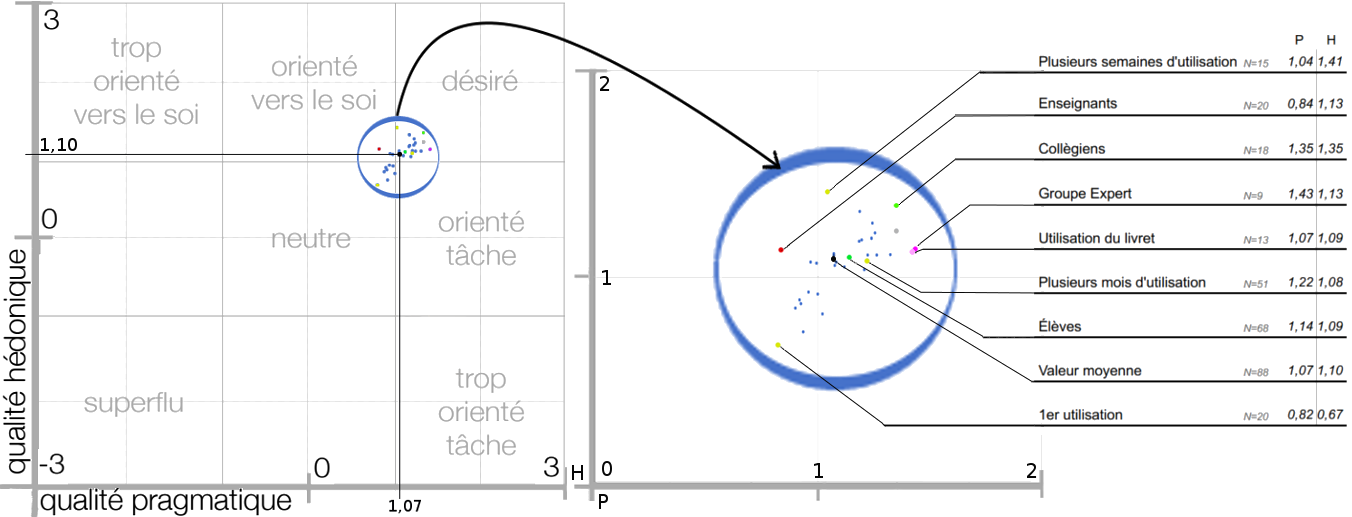
\includegraphics[width=0.9\linewidth]{Figures/Desprez_didapro-attrakdiff_point.png}
            \caption{Résultats \textit{AttrakDiff}, réduits à deux dimensions.}\label{fig:attrakdiff_point}
        \end{figure}\par%
        Tout d'abord nous pouvons observer que le groupe d'enseignants s'écarte significativement ($p=0,0564$, $ddl=28$) du groupe des élèves  ($Test\ de\ Student\ bilat\acute{e}ral\;\ \alpha=0,05\;\ ref\ var=\acute{E}l\grave{e}ves$), évaluant globalement la plateforme comme plus \gui{orientée~vers~le~soi} mais principalement causé par un score plus faible sur l'axe $x$ noté $P$ \gui{qualité pragmatique} ($p=0,00002$, $ddl=14$) (sur l'axe $y$ noté $H$ \gui{qualité hédonique} $p=0.7359$, $ddl=14$).
        Ceci peut être induit par la stratégie de conception qui plaçait les besoins \tiret{et~envies} de l'utilisateur au centre du développement.
        De plus l'enseignant adaptant le dispositif aux objectifs théoriques et pratiques qu'il s'est fixé, il semble cohérent que le score sur l'échelle pragmatique soit plus élevé chez les élèves, manipulant \textit{in~fine} le dispositif modifié par l'enseignant pour les besoins de la tâche ou du TP.
        Ensuite nous pouvons remarquer que le temps total d'utilisation de la plateforme modifie les résultats.
        Ainsi, manipuler le kit pour la première fois provoque une moyenne des réponses significativement plus neutre ($p=0,0000$), tandis que nous observons, pour le groupe l'ayant utilisé pendant plusieurs semaines, des valeurs significativement plus positives ($p=0,0004$) sur $H$;
        le groupe pratiquant depuis plusieurs mois est lui beaucoup plus proche de la la moyenne mais reste significativement différent sur $P$ ($p=0,0006$) et donc plus \gui{orienté vers la tâche}.
        De plus cette proximité avec la moyenne pourrait s'expliquer par l'effectif important de cette sous-catégorie d'élèves.
        Un autre fait remarquable se situe au niveau de la modalité \gui{utilise le livret pédagogique fourni} et le groupe \gui{Expert} qui obtiennent une évaluation similaire sur les deux échelles ($p=0,9469$) et qui est significativement différente de la moyenne sur $H$ et $P$ pour la modalité \gui{livret} ($p=0,0011$) mais uniquement sur $P$ ($p=0,0039$) pour les \gui{experts}.
        Enfin nous observons que le groupe des collégiens possède la meilleure évaluation globale, même si, individuellement ces moyennes sur les différentes échelles ne correspondent pas systématiquement à la valeur maximale.
    \subsection{Dans d'autres contextes}\label{Exp:vs_thymio}
        \paragraph{Introduction}
            Dans un second temps, il est intéressant d'observer et de mesurer l'utilisabilité du kit ErgoJr face à d'autres kits pédagogiques et surtout dans d'autres contextes. À noter qu'avec l'entrée de l'informatique dans le tronc commun des lycéens~\citeS{sec:programme-officiel} le besoin d'enseignant formé à cette matière pluridisciplinaire croit plus rapidement que annoncé. Ainsi, l'offre de formation \tiret{y compris en robotique} croit également, rendant l'étude de ce contexte pertinent. De plus, étant donné que l'élève représente une cible secondaire accessible uniquement via son enseignant~\citeS{sec:user_cible}, il semblait donc particulièrement intéressant d'éprouver notre kit dans un contexte de formation professionnelle.
        \paragraph{Méthode}
            Deux sessions de formation en robotique ont été organisées. Chacune dispensée sur une journée de 6~heures à des groupes de 16 adultes engagés dans une formation de deux semaines sur le numérique. Cette journée de robotique se divisait en deux: la matinée consacrée au robot Thymio, l'après-midi consacrée au robot Poppy ErgoJr. Les participants étaient invités à constituer librement des groupes de deux personnes pour l'ensemble des activités de la journée.
            Chaque demi-journée se clôturait par la passation individuelle de deux questionnaires validés: le \sht{SUS} et l' \sht{ATT}, rendant compte respectivement de l'utilisabilité et de l'expérience utilisateur.
            Aucune donnée personnelle sur les participants n'a été recueillie, et un total de 29 réponses complètes ont été collectées.
            \subparagraph{Déroulement des activités}
                Pour cette journée, il a été demandé au formateur de définir un robot comme étant une composition de capteurs et d'effecteurs associés à un micro-contrôleur contenant sa programmation et que de son interaction avec l'environnement émergeait un comportement. Le second objectif était d'introduire des notions élémentaires de la programmation, à savoir, les conditions et les boucles.
                %thymio
                Les activités de la matinée étaient constituées des missions 1, 2, 3, 4 puis la mission 10 extraite du parcours \textit{IniRobot}~\citeB{roy2016inirobot}. Les deux premières se focalisent sur l'observation et la découverte du robot face à 4 comportements pré-programmés. Les documents fournis viennent les guider vers un formalisme \textit{Si~\dots Alors~\dots} (\eg en mode jaune, si je mets un obstacle à gauche alors Thymio tourne à droite). À partir de la mission 3,\sht{vpl} est introduit. Ce langage de programmation événementiel et entièrement visuel propose de manipuler 2 types de cartes (\eg cartes capteurs et effecteurs) à associer via le formalisme \textit{Si~\dots Alors~\dots} sur la zone de script centrale~\citeT{tab:langue}. La mission 10 était consacrée à la réalisation d'un parcours d'obstacles présentés comme un défi où les participants sont invités à coder un programme similaire au comportement explorateur (mode jaune) observé durant les missions précédentes.
                %ergo
                Les activités de l'après-midi étaient constituées de deux activités de découverte pour le robot ErgoJr: l'activité \textit{caméléon}~\citeA{pdf:act_cameleon}focalisée sur les capteurs et l'activité \textit{chamboule~tout}~\citeA{pdf:act_chamboul} focalisée sur les effecteurs.
                La première partie de l'activité \textit{caméléon} est destinée à la prise en main de l'interface \sht{snap}~\citeT{tab:langue} et des principes de la programmation visuelle par bloc~\citeB{harvey2012snap}: mode d'interaction par cliquer/déposer, activation de plusieurs séquences d'instructions en parallèles, typage des blocs, \etc. La seconde partie propose un défi où l'objectif est de faire varier la couleur des leds présentes sur le robot en fonction d'un set de couleurs présenté successivement devant sa caméra.
                L'activité \textit{chamboule~tout} propose de découvrir la méthode de contrôle des servo-moteurs, à savoir, le mode \textit{compliant} qui permet de déplacer les moteurs avec les mains \textit{versus} le mode \textit{stiff} permettant d'envoyer des instructions \cro{en position} aux 6 moteurs via les blocs \sht{snap}. Il est ensuite proposé aux participants de réaliser un programme permettant au robot ErgoJr de propulser une balle en direction d'une pile de gobelets.
        \paragraph{Résultats}
            \subparagraph{Qualitativement},
                l'ensemble des participants ont réussi tous les objectifs fixés avec les deux robots et ont déclaré verbalement aux formateurs leur satisfaction à avoir participé à cette journée.
            \subparagraph{Quantitativement},
                nous pouvons observer sur la figure~\ref{fig:sus_vs_thymio} que les 4 trajectoires présentées semblent identiques, avec un décalage en faveur du robot Thymio. Ce décalage est particulièrement visible sur le 4\ieme item. Nous constatons également un score très faible pour cette formation sur le 1\ier item au regard des résultats obtenus en 2017. Mais ceci, s'explique par leurs contextes distincts.\par%
                Un test t de Student pour deux échantillons appariés a été réalisé entre les résultats du Thymio et ceux du Poppy ErgoJr durant cette formation. Il montre effectivement un score significativement supérieur pour le Thymio ($p=2.6e-6$). Cependant, un test t de Student pour deux échantillons indépendants montre que la différence entre les résultats du Thymio et les résultats de 2017 du Poppy ErgoJr n'est pas significative ($p=0.34$).
                \begin{figure}[!h]
                    \centering
                    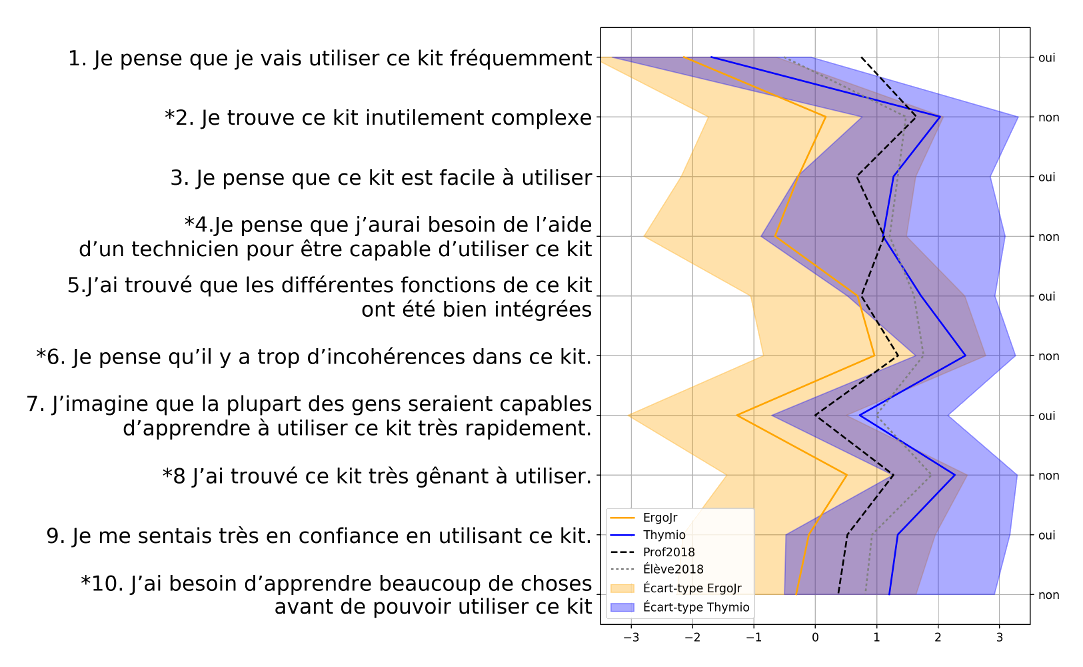
\includegraphics[width=0.9\linewidth]{Figures/Desprez_eiah-sus.png}
                    \caption{Résultats SUS ErgoJr et Thymio~\citeB{desprez:hal-02120958}}\label{fig:sus_vs_thymio}
                \end{figure}\par%
                \begin{figure}[!h]
                    \centering
                    \label{fig:att_vs_thymio}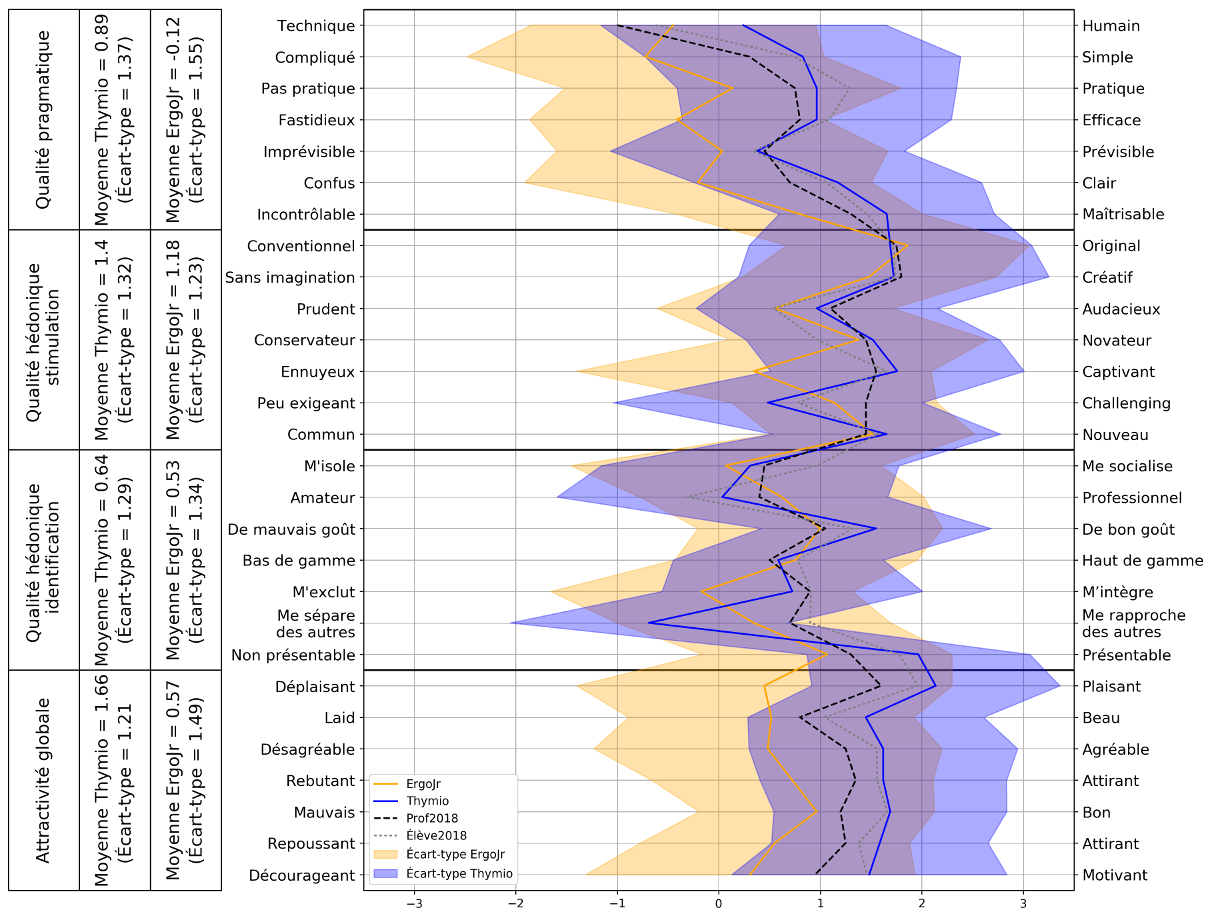
\includegraphics[width=0.9\linewidth]{Figures/Desprez_eiah-atrakdiff.png}
                    \caption{Résultats \textit{AttrakDiff} ErgoJr et Thymio~\citeB{desprez:hal-02120958}}
                \end{figure}\par%
                Le constat est sensiblement identique à celui du SUS: Les résultats sont significativement meilleurs pour le Thymio face au Poppy ErgoJr dans ce contexte de formation ($p=8.36e-5$) mais pas significativement face aux résultats de 2017 ($p=0.34$).
                De plus, nous constatons que c'est principalement sur la 1\iere~et la 4\ieme~échelle qu'est portée cette différence,  et que d'un point de vue uniquement hédonique, aucune plateforme ne se distingue.
    \subsection{Synthèse}
        Ces deux questionnaires \tiret{standardisés} nous ont permis, d'une part de rassembler un certain nombre d'éléments quantifiables afin de mieux évaluer les choix et stratégies de conception pris pour le dispositif Poppy Éducation et ce, principalement sur le kit ErgoJr.
        Cela nous permet de mieux appréhender la pertinence des solutions proposées en fonction des différents usages et perceptions qu'ont les utilisateurs.
        D'autre part, utiliser ces questionnaires nous permet de proposer une \gui{photographie} des caractéristiques d'utilisabilité perçues par l'utilisateur selon différents critères.
        Ceci offre la possibilité de comparaisons futures avec d'autres dispositifs de robotique pédagogique, permettant de mieux classifier ces outils.
        Mais déjà, nous constatons que tant sur l'utilisabilité que sur l'expérience utilisateur, relevées respectivement par le \sht{SUS} et l' \sht{ATT}, nous observons de meilleurs résultats pour le Thymio dans un contexte de formation courte chez un public novice. Cependant, placé dans le contexte pour lequel il a été conçu, c'est à dire, de façon répétée en classe par un public d'élèves et d'enseignants ayant déjà exploré les rudiments de la programmation, le Poppy ErgoJr a obtenu des résultats comparables à celui du Thymio. De plus, au niveau de l'expérience utilisateur les caractéristiques hédoniques des deux plateformes obtiennent des scores similaires, indépendamment du contexte. Ainsi, ces résultats tendent à montrer que le Thymio est plus adapté à l'initiation d'un public novice, là où le Poppy~ErgoJr serait plus adapté à l'approfondissement, et que tous deux sont des plateformes robustes en terme d'utilisabilité. % utilisabilité
%PART_3_CHAP_3_SEC_2
%WAIT a Review, ok
\clearpage
\section{Acceptabilité}\label{Exp:L_ACC}
    \subsection{Introduction}
        L’utilisabilité d’un système ne crée pas nécessairement son acceptation~\citeS{sec:acceptable}; de plus, ici nous ne traiterons pas de l'acceptabilité des kits robotiques pédagogiques à l'école en elle-même, mais de l'impact de ces kits (en l'occurrence du kit ErgoJr) sur les perceptions sociétales des individus, et donc sur l'acceptabilité de la robotique en générale, d'où le recours au questionnaire \sbg{EURO382} durant notre étude longitudinale; et au questionnaire \sht{NARS} dans une seconde étude ponctuelle.
    \subsection{Attitude toward robot (Euro382)}\label{Exp:euro}
        \paragraph{Méthode}
            Durant l'année scolaire 2016-2017, 68 élèves et 19 enseignants ont pratiqué des activités robotiques de différentes natures, et ont complété, en juin, le questionnaire \sht{EURO382}~\citeA{pdf:EURO382}. 146 élèves et 9 enseignants n'ayant pratiqué aucune activité robotique ont complété également ce questionnaire.
            Une 1\iere hypothèse est d'observer une différence entre les résultats globaux de 2012 et ceux de 2017 traduisant une acceptabilité accrue de la robotique.
            Un 2\ieme porte sur la distinction élèves, enseignants. Cette distinction pourrait avoir deux facteurs principaux: la fonction (enseignant~/~élève) ou l'âge. Pour estimer cette effet d'âge nous avons à disposition les résultats de 2012 concernant les 15-24 ans comparés au 40-54 ans.
            Une 3\ieme sur l'impact induit par la pratique d'activités robotiques. Notamment une meilleure acceptation.
            Une 4\ieme s'intéresse aux caractéristiques des activités, notamment le fait d'utiliser le livret pédagogique.
            Enfin, une 5\ieme hypothèse porte sur la distinction homme, femme, qui bien que souvent présente dans les disciplines scolaires scientifiques semble s'atténuer, voire disparaître, dans le contexte d'activités robotiques.
            \subparagraph{Population}
                En 2012 plus de 1000 personnes de chaque pays de l'union européenne ont passé ce questionnaire. Les résultats étant publiques nous pouvons les comparer avec notre échantillon constitué de $28$ enseignants et $146$ élèves de la région Nouvelle Aquitaine ayant complété ce même questionnaire (en classe \etou en ligne) durant le mois de juin 2017.
                Sur chacune des figures présentant les résultats~\citeA{pdf:euro_result} à chacune des \sht{ques} de \sht{EURO382}\citeA{pdf:EURO382}, nous pouvons repérer les modalités issues des résultats des passations de 2012, à savoir: les résultats pour la population française ($N=1059$), la population du sud-ouest ($N=120$), la population des 40-50 ans ($N=266$), la population des 15-24 ans ($N=159$), la population d'hommes français ($N=505$), la population de femmes françaises ($N=554$); toutes identifiées par~une~*. En plus de ces modalités de 2012, nous retrouvons sur nos figures l'ensemble des modalités qui ont été définies pour les besoins de notre étude. %\url{https://data.europa.eu}
                Ici, nous étudions plusieurs groupes d'individus: les enseignants et les élèves. Parmi les élèves nous nous intéressons à ceux ayant pratiqué des activités avec le kit ErgoJr ($N=68$). Ces $68$ élèves sont ensuite répartis dans différentes modalités suivant les caractéristiques des activités qu'ils ont suivi: ils peuvent avoir déclaré utiliser le livret pédagogique~\citeB{noirpoudre2016livret} fourni dans le kit ($N=13$) ou non ($N=55$); avoir utilisé d'autres kits robotiques ($N=16$); avoir pratiqué moins de 6~heures d'activités avec le robot ($N=30$), entre 6 et 25~heures ($N=22$) ou plus de 25~heures ($N=16$); avoir construit le robot ($N=12$); avoir utilisé le langage de programmation visuel \sht{snap} ($N=46$), le langage de programmation textuel \textit{Python} ($N=21$), les deux ($N=8$) ou aucun ($N=9$), il est à noter que ces deux langages sont directement accessibles via l'interface principale du robot. Les résultats présentent également les populations d'enseignants et d'élèves (ayant pratiqué ou non des activités) en fonction de leur genre, à savoir: $21$ enseignants (dont $15$ \sht{EP}), $7$ enseignantes (dont $4$ \sht{EP}), $118$ élèves garçon (dont $44$ \sht{EP}) et $96$ élèves fille (dont $24$ \sht{EP}).
        \paragraph{Résultats descriptifs}
          \subparagraph{Évolution temporelle.}
            Nous constatons des évolutions entre les passations réalisées en 2012 ($N=1059$) et nos passations de Juin 2017 ($N=242$ dont $21$ enseignants).
            De plus, les résultats régionaux (\ie Sud-ouest) de 2012 ($N=120$) sont également présentés afin d'illustrer les variations locales.
            En premier lieu, nous constatons que l'attrait pour les nouvelles technologies~\citeQ{1} est plus fort aujourd'hui, la part des \textit{très intéressé} passant de 34 à 53\prc[.]
            En revanche, sur la 2\ieme \sht{ques}, l'évolution n'est que partielle. 
            En effet, l'image du bras industriel correspond, pour le répondant, à la robotique, dans les mêmes proportions qu'en 2012 (environ 85\prc de réponses positives); alors que l'image du robot domestique humanoïde connaît une progression avec environ 75\prc en 2017 contre environ 55\prc en 2012.
                \begin{figure}[!h]
                    \begin{minipage}{0.45\linewidth}
                    \subcaption{\label{fig:QI2-1} Robot, bras industriel}
                    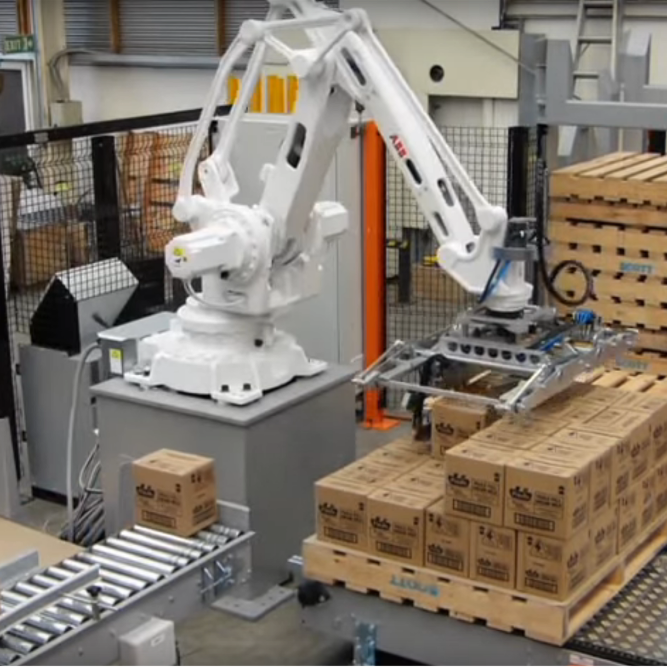
\includegraphics[width=\linewidth]{Figures/Euro-QI2_1}
                    \end{minipage}
                    \hfill
                    \begin{minipage}{0.45\linewidth}
                    \subcaption{\label{fig:QI2-2} Robot, humanoïde}
                    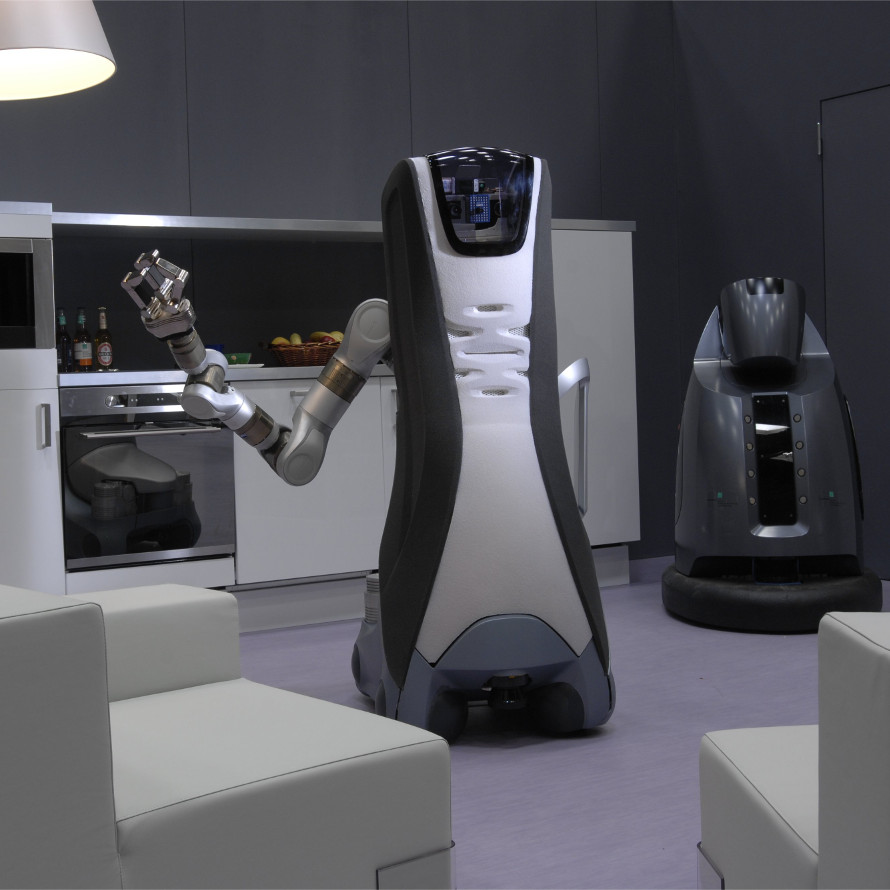
\includegraphics[width=\linewidth]{Figures/Euro-QI2_2}
                    \end{minipage}
                    \caption{Les robots visibles dans le questionnaire Euro382}
                \end{figure}
            Cependant, cette progression est à relativiser car notre échantillon, principalement constitué d'élèves (88\prc[)], obtient des scores correspondant aux 15-24 en 2012.
            La~\sht{ques}3 ({\footnotesize page~\pageref{QA3}}) montre un progression à la faveur du \textit{oui à la maison} passant de environ 10 à 25\prc et du \textit{oui~ailleurs} passant de 1 à 6\prc[.]
            Nous voyons, grâce à la~\sht{ques}4 ({\footnotesize page~\pageref{QA4}}), qu'en 5~ans, l'image que pense avoir les répondants de la robotique s'est améliorée, avec une quasi disparition de la réponse \textit{très négative}.
            Cela s'observe aussi dans la~\sht{ques}5 avec davantage d'accords sur le fait que \textit{les robots aident les gens}~\citeQ{5-1} et davantage de désaccords avec le fait que \textit{les robots volent des emplois }({\footnotesize page~\pageref{QA5-2}}).
            En revanche, il y a peu d'évolution d'opinion sur la nécessité \textit{des robots pour accomplir des tâches dangereuses ou difficiles} (massivement oui~\citeQ{5-3}), et sur \textit{la gestion prudente qu'il faut avoir vis-à-vis des robots} (massivement oui~\citeQ{5-4}). 
            Une forte évolution, concerne l'impact perçu par l'utilisation de robots sur la création d'emplois~\citeQ{5-5} qui est davantage vue comme stimulateur (avec également une forte progression des \sht{NSP} passant d'environ 10 à 20\prc[)].
            Pour la~\sht{ques}6 ({\footnotesize page~\pageref{QA6}}), nous constatons une légère progression des domaines \cro{civils} (\ie usage domestique, transport, agriculture) au dépend des activités \cro{d'État} (\ie domaine militaire, sécurité et recherche, exploration spatiale). Cependant nous retrouvons des propensions globalement identiques entre 2012 et 2017.
            En revanche, concernant la~\sht{ques}7 ({\footnotesize page~\pageref{QA7}}), nous observons une très large progression de la catégorie \cro{\textit{aucun}} (0\prc en 2012 contre 7\prc en 2017).
            Les résultats à ces deux~\sht{ques} pourraient être la traduction d'une meilleure acceptabilité de la robotique et de sa généralisation dans de nombreux usages du quotidien.
            La~\sht{ques}8, se décline en 4 sous-questions et traite de cette notion d'acceptation au quotidien pour 3 domaines: la santé, les services domestiques et le travail.
            Nous constatons un décalage entre 2012 et 2017:\textit{ se faire opérer par un robot}~\citeQ{8-1}, \textit{faire promener son chien}~\citeQ{8-2}, ou \textit{faire garder son enfant}~\citeQ{8-4} sont des situations moins inacceptables, respectivement: 13, 9, $<$2,5\prc de \textit{tout~à~fait mal~à~l'aise} en 2017 contre 38, 61 et 85\prc en 2012.
            En revanche, \textit{être assisté par un robot au travail}~\citeQ{8-3} donne des résultats plus tranchés en 2017, avec une légère majorité de réponses négatives (\ie \textit{tout~à~fait mal~à~l'aise}. 
            Nous pouvons aussi noter la disparition des catégories \textit{pas applicable} et \sht{NSP}.
            Enfin, concernant les prévisions d'une généralisation des robots domestiques~\citeQ{9}, si aucune évolution n'est relevée, un simple décalage des réponses correspondant au laps de temps entre les 2 passations (5 ans) devrait s'observer.
            Mais, moins de 2\prc estimaient en 2012 que cela était chose courante, et 12\prc que cela serait chose courante en 2017, alors qu'ils sont aujourd'hui 7\prc à considérer que cela est chose courante. Plus globalement, ils étaient environ 60\prc à estimer cette généralisation à moins de 20 ans, aujourd'hui, 5 ans après, ils sont environ 70\prc à l'estimer à moins de 10 ans. Nous constatons donc un rapprochement de l'échéance perçue par les individus sur cette~\sht{ques}.
            %%%%%%%%%%%%%%%%%%%%%%%%%%%%%%%%%%%%%%%%%%%%%%%%%%%%%%%
          \subparagraph{Distinction élèves et enseignants.}
            Afin d'illustrer l'influence de l'âge dans ces distinctions, sur  les distinctions entre les $214$ élèves et les $28$ enseignants ayant répondu, les résultats de 2012 des 40-50 ans ($N=266$) et des 15-24 ans ($N=159$) sont également présentés.
            Une première constatation est que les enseignants sont davantage intéressés par cette thématique~\citeQ{1} (75\prc de \textit{très intéressé}, contre 50\prc chez les élèves). Cependant, cet écart se retrouve aussi dans les résultats de 2012 d'où un probable effet d'âge. 
            Il en est de même pour les 2~images où l'écart ici observé est similaire à 2012 entre ces deux classes d'âges ({\footnotesize page~\pageref{QA2-1}}).
            En revanche, pour la 3\ieme \sht{ques}({\footnotesize page~\pageref{QA3}}) les tendances s'inversent: les élèves se déclarent plus utilisateurs de robots (38\prc \textit{total oui}) que ne le déclarent les enseignants (35\prc[)] notamment \textit{à~la~maison} (27\prc contre 16\prc[)], alors qu'en 2012, les plus âgés étaient ceux se déclarant le plus utilisateur (\textit{total oui}: 21\prc des 40-54 ans, contre 15\prc des 15-24 ans).
            Cette inversion s'observe également sur la~\sht{ques}4 ({\footnotesize page~\pageref{QA4}}): en 2017, les plus âgés de l'échantillon, les enseignants, qui ont un avis majoritairement pro-robot.
            Aux 5~\sht{aff} de la~\sht{ques}5, nous observons que les enseignants ont un avis qui suis la même tendance que l'évolution des réponses entre 2012 et 2017, mais avec des traits plus marqués. 
            Notamment, sur la 2\ieme \sht{aff} avec 60\prc de désaccords~\citeQ{5-2}; à l' \sht{aff}3 avec 100\prc d'accords~\citeQ{5-3}; et à l' \sht{aff} 1 et 5 avec l'absence de réponse \textit{pas~du~tout~d'accord} ({\footnotesize page~\pageref{QA5-1}~et~\pageref{QA5-5}}).
            Cependant, pour la 4\ieme \sht{aff}, seuls 86\prc des enseignants sont en accord avec la nécessité de \textit{gérer avec prudence} les robots contre 94\prc des élèves et 95\prc en 2012~\citeQ{5-4}.
            Concernant les domaines d'activités préconisés ou proscrits par les répondants pour les robots  ({\footnotesize page~\pageref{QA6}~et~\pageref{QA7}}), nous constatons des réponses similaires chez les enseignants et les élèves, comme l'étaient celles des jeunes et âgés en 2012. À noter, le recul de la préconisation du domaine militaire par les enseignants (moins de 2,5\prc contre 12\prc chez les élèves et 14\prc en 2012).
            Comme pour la 5\ieme \sht{ques}, les enseignants suivent une tendance identique à celle des élèves: une meilleure acceptation de la robotique ({\footnotesize page~\pageref{QA8-1},~\pageref{QA8-2}~et~\pageref{QA8-4}}), avec 2 nuances: sur la 3\ieme \sht{aff}, 54\prc de \textit{tout~à~fait mal~à~l'aise} contre 26\prc chez les élèves et 13\prc en 2012 ({\footnotesize page~\pageref{QA8-3}}); et sur la 1\iere \sht{aff}, la distinction entre enseignants et élèves de 2017 s'inverse par rapport à celle observée entre les 40-54 et les 15-24 ans en 2012: les jeunes étaient davantage \textit{mal~à~l'aise}, aujourd'hui ce sont les enseignants.
            En outre, à la 3\ieme \sht{aff}, nous voyons apparaître une distinction entre élèves et enseignants, là où en 2012 les résultats des 14-25 ans et des 40-54 ans étaient similaires.
            Enfin, à la~\sht{ques}9 ({\footnotesize page~\pageref{QA9}}), une même évolution est constatée entre élèves et enseignants mais plus exacerbée: 79\prc des enseignants estimaient que les robots domestiques seront \textit{une chose courante dans 10 ans ou moins} contre 66\prc des élèves. Mais surtout, ils sont 0\prc à l'estimer \textit{dans plus de 20 ans} (contre 8\prc des élèves).
            %%%%%%%%%%%%%%%%%%%%%%%%%%%%%%%%%%%%%%%%%%%%%%%%%%%%%%%
          \subparagraph{Distinction avec et sans activité robotique.}
            Des distinctions entre les réponses des $68$ \sht{EP} et celles des $146$ \sht{ENP}.
            En effet, dès la 1\iere \sht{ques}({\footnotesize page~\pageref{QA1}}), nous observons qu'aucun des \sht{EP} se déclare \textit{pas du tout intéressé} par les nouvelles technologies contre 4\prc des \sht{ENP}, et qu'ils ont un intérêt déclaré supérieur (57 contre 47\prc[)]. 
            %nous pouvons noter que seules les étudiantes \sht{ENP} obtiennent un score plutôt faible 31\prc mais comparable à ceux obtenus en moyenne en 2012.
            Pour la 1\iere image~\citeF{fig:QI2-1} pas de différence entre les \sht{EP} et les \sht{ENP}. 
            En revanche, pour la 2\nde avec le robot humanoïde~\citeF{fig:QI2-2}, nous voyons une progression des \sht{NSP} chez les \sht{EP} (13\prc[)] et pas chez les \sht{ENP} (2\prc[)].
            La 3\ieme \sht{ques}({\footnotesize page~\pageref{QA3}}) montre de légères différences là où nous aurions attendu avoir une forte distinction:
            la principale concerne la propension de ceux ayant répondu \textit{oui~à~la~maison} étant de 30\prc chez les \sht{ENP} contre 19\prc chez les \sht{EP}, cet écart est au profit du \textit{oui ailleurs} étant de 3\prc chez les \sht{ENP} contre 14\prc chez les \sht{EP}, soit 36\prc \textit{oui} tout confondu pour les \sht{ENP} et 38\prc pour les \sht{EP}.
            À noter aussi, une plus forte présence du \sht{NSP} pour les \sht{EP}: 7\prc contre 2\prc[.]
            À la~\sht{ques}4 ({\footnotesize page~\pageref{QA4}}), nous observons que les \sht{EP} ont un \textit{à priori} que les \sht{ENP} n'ont pas (moins de 2\prc d'avis négatifs contre 14\prc des \sht{ENP}).
            À la 1\iere \sht{aff}({\footnotesize page~\pageref{QA5-1}}), nous constatons que environ 90\prc des élèves s'accordent à dire que \textit{les robots sont une bonne chose pour la société} mais de manière moins radicale chez les \sht{ENP}: 20\prc de \textit{Tout~à~fait~d'accord} contre 37\prc chez les \sht{ENP}.
            À l'inverse, sur la 2\ieme \sht{aff}({\footnotesize page~\pageref{QA5-2}}) la radicalité s'observe chez les \sht{EP}: environ 45\prc des élèves sont en désaccord avec l'idée que \textit{les robots volent les emplois} et seuls 10\prc des \sht{ENP} ne sont \textit{pas~du~tout~d'accord}, contre 21\prc des \sht{EP}.
            Concernant \textit{la nécessité des robots pour les taĉhes dangereuses}~\citeQ{5-3}, nous notons une propension légèrement supérieure d'accords chez les \sht{EP} (89\prc contre 86\prc[)] et l'apparition de la réponse \sht{NSP} à hauteur de 3\prc contre 0\prc[)].
            Pour \textit{la gestion prudente de cette technologie}~\citeQ{5-4} c'est pour les \sht{ENP} que nous constatons un accord légèrement supérieur: 95\prc contre 94\prc[.]
            Concernant la \textit{stimulation de la création d'emploi}~\citeQ{5-5}, nous observons une plus nette distinction, les \sht{EP} étant majoritairement en accord (56\prc[)] ce qui n'est pas le cas chez les \sht{ENP}: 41\prc d'accord. Nous constatons également chez ces 2 groupes une forte présence de la réponse \sht{NSP} (environ 21\prc[)].
            Au niveau des domaines d'activités préconisées et à proscrire ({\footnotesize page~\pageref{QA6}~et~\pageref{QA7}}), les \sht{EP} et les \sht{ENP} ont des résultats globalement identiques, sauf pour le domaine à proscrire \cro{\textit{aucun}} où les \sht{EP} semblent plus proches des enseignants que des \sht{ENP}: respectivement 9, 11 et 5\prc[.]
            Globalement, sur les aspects abordés dans les~\sht{ques} de la 8\ieme \sht{ques}, nous pouvons noter un ressenti légèrement plus positif côté \sht{EP}, avec des réponses égales à 9 \etou 10 (0 = \textit{tout~à~fait mal~à~l'aise} et 10 = \textit{tout~à~fait à~l'aise}) plus fréquentes pour ces 4~\sht{ques}({\footnotesize page~\pageref{QA8-1},~\pageref{QA8-2},~\pageref{QA8-3}~et~\pageref{QA8-4}}). 
            Cet aspect pourrait montrer l'impact de la pratique d'activités pédagogiques sur l'acceptabilité de la robotique. De plus, la présence accrue de réponses \sht{NSP} pourrait traduire une prise de conscience chez les \sht{EP} d'une vision plus complexe de la robotique.
            Sur les perspectives de \textit{généralisation de la robotique domestique} les \sht{EP} semblent être plus précis: 46\prc l'estiment à \textit{10 ans}, les \sht{ENP} semblant plus indécis (résultats plus distribués). Pour ces 2 groupes, environ 8\prc pensent que \textit{c'est déjà une chose courante} et 4\prc ne se prononcent pas.
            %%%%%%%%%%%%%%%%%%%%%%%%%%%%%%%%%%%%%%%%%%%%%%%%%%%%%%%
          \subparagraph{Distinction entre les caractéristiques des activités.}
            Nous constatons des distinctions issues des caractéristiques des activités proposées par les enseignants aux $68$ élèves ayant complété le questionnaire. 
            Cependant, même si ces modalités ont révélé avoir un impact, celui-ci reste localisé; aucune des modalités n'offrant de distinction significative sur l'ensemble des~\sht{ques} du questionnaire.
            Concernant la 1\iere \sht{ques}({\footnotesize page~\pageref{QA1}}), nous constatons que les élèves n'ayant pas utilisé les langages de programmation par défaut (\sht{snap} et \textit{Python}) ont un score bien inférieur aux autres (11\prc[)] et que les élèves \sht{ENP} avec \sht{snap} ont également un score faible 36\prc comparé à la moyenne de notre échantillon 53\prc[.]
            Pour la 2\ieme, c'est la modalité \textit{utilise un autre kit} qui offre une distinction notamment pour la 1\iere image~\citeF{fig:QI2-1} correspondant davantage à la représentation de robot pour eux (44\prc contre 19\prc en moye nne).
            Sur la 2\nde~image~\citeF{fig:QI2-2} on note la forte présence des réponses \sht{NSP} dans certaines modalités (13\prc en moyenne avec des pics allant jusqu'à 21\prc[)], mais aussi son absence dans les modalités \textit{avec livret} et \textit{utilise \sht{snap} et python}.
            Sur la~\sht{ques}3 ({\footnotesize page~\pageref{QA3}}), un ensemble de facteurs semble déterminer l'apparition de la réponse \sht{NSP}: le fait d'avoir utilisé le livret pédagogique, d'avoir construit le robot, d'avoir utilisé le langage de programmation textuel \textit{Python} et d'avoir plus de 25h de pratique, fait tendre les \sht{NSP} vers 0. À noter également, que les répondants des modalités \textit{utilisent d'autres kits} et \textit{plus de 25h de pratique} ont un taux de \textit{oui} plus élevé (environ 50\prc[)] que la moyenne des \sht{EP} (38\prc[)].
            Sur les \textit{à priori}~\citeQ{4}, ils sont plutôt \textit{très positifs} pour la modalité \textit{avec livret} et \textit{utilise \sht{snap} et Python} (46 et 62\prc contre 28\prc en moyenne), avec une niche de réponses \textit{plutôt négatif} dans la modalité \textit{n'utilise ni \sht{snap}, ni Python} (11\prc contre moins de 2,5\prc en moyenne).
            À la 1\iere \sht{aff} de la~\sht{ques}5 ({\footnotesize page~\pageref{QA5-1}}), la modalité \textit{avec livret} se démarque avec 62\prc d'accord contre 37\prc en moyenne. L'absence de désaccord pour les modalités \textit{utilise Python} et \textit{entre 6 et 25h de pratique} est aussi à noter.
            À la 2\ieme \sht{aff}({\footnotesize page~\pageref{QA5-2}}), ici encore c'est la modalité \textit{avec livret} qui totalise l'accord le plus grand (31\prc contre 12\prc en moyenne), mais aussi le désaccord le plus grand (38\prc contre 21\prc[)] ex~aequo avec la modalité \textit{utilise \sht{snap} et Python} qui, de plus, est la 2\nde~modalité où la réponse \sht{NSP} est la plus présente (12\prc contre 4\prc[)] et la seule marquée par l'absence de réponse \textit{tout~à~fait~d'accord}.
            À la 3\ieme \sht{aff}({\footnotesize page~\pageref{QA5-3}}), nous retrouvons une majorité d'accords et une absence de désaccords pour les modalités \textit{avec livret} et \textit{utilise \sht{snap} et Python} (69 et 88\prc contre 57\prc en moyenne). Nous notons aussi, une forte présence des \sht{NSP} dans la modalité \textit{ni \sht{snap}, ni Python} (11\prc contre 3\prc[)].
            À la 4\ieme \sht{aff}({\footnotesize page~\pageref{QA5-4}}), une nouvelle fois, c'est la modalité \textit{à construit le robot} qui totalise le plus de réponses \sht{NSP} (9\prc contre moins de 2,5\prc[)] et la modalité \textit{utilise \sht{snap} et Python} pour la réponse \textit{tout~à~fait~d'accord} (75\prc contre 49\prc[)].
            Le maximum de désaccords est atteint par la modalité \textit{à construit le robot} avec 17\prc de \textit{plutôt~pas~d'accord} talonné par la modalité \textit{avec livret} à 15\prc[.]
            À la 5\ieme \sht{aff}({\footnotesize page~\pageref{QA5-5}}), nous constatons que les modalités \textit{utilise \sht{snap} et Python} et \textit{n'utilise ni \sht{snap}, ni Python} sont les seules à ne totaliser aucune réponse \sht{NSP} là où toutes les autres avoisinent les 20\prc[.] À noter également, l'absence de désaccords pour les 4 modalités \textit{avec livret, plus de 25h de pratique, à construit le robot} et \textit{utilise \sht{snap} et Python} contre 7\prc en moyenne. Cette dernière modalité est ici encore la modalité totalisant le plus de réponses \textit{tout~à~fait d'accord} (50\prc contre 18\prc en moyenne).
            Concernant les domaines d'activités préconisés et à proscrire ({\footnotesize page~\pageref{QA6}~et~\pageref{QA7}}), le nombre de réponses possibles (3 parmi 12 soit 220 possibilités) associé à un effectif relativement faible dans certaines modalités ($Min=8$) ne permet pas la mise en évidence de variations suffisamment importantes.
            Au niveau du ressenti abordé en~\sht{ques}8, nous constatons à la 1\iere \sht{aff}({\footnotesize page~\pageref{QA8-1}}) que, là encore, les modalités \textit{avec livret} et \textit{utilise \sht{snap} et Python} offrent les réponses les plus saillantes: cette 1\iere modalité montrant une meilleure acceptation (38\prc de réponses supérieures à 8 points, contre 18\prc en moyenne); à l'inverse, la 2\nde, montre une acceptation plus faible (63\prc de réponses inférieures à 3, contre 34\prc[)].
            À la 2\ieme \sht{aff}({\footnotesize page~\pageref{QA8-2}}), nous notons principalement le total des réponses supérieures à 7 atteignant 42\prc dans la modalité \textit{a construit le robot} contre 17\prc en moyenne.
            À la 3\ieme \sht{aff}({\footnotesize page~\pageref{QA8-3}}), nous constatons que les scores (\textit{tout~à~fait mal~à~l'aise}) pour les modalités \textit{avec livret, à construit le robot} et \textit{utilise \sht{snap} et Python} sont plus similaires à ceux des enseignants qu'à ceux des autres élèves, respectivement: 46, 33, 50\prc pour ces 3~modalités, 54\prc pour les enseignants, 26\prc pour les élèves contre 13\prc en 2012.
            À la 4\ieme \sht{aff}({\footnotesize page~\pageref{QA8-4}}), c'est encore la modalité \textit{a construit le robot} qui montre la plus grande acceptation de la robotique (33\prc de réponses supérieures à 7, contre 16\prc en moyenne).
            Enfin, la 9\ieme \sht{ques}({\footnotesize page~\pageref{QA9}}) montre une nette différence pour la modalité \textit{avec livret} où \textit{la généralisation de la robotique dans les tâches ménagères} n'est pas envisagée avant \textit{20 ans ou plus} pour 61\prc[,] contre 25\prc en moyenne. Une tendance similaire pour la modalité \textit{a construit le robot} est observée (42\prc[)], nous notons aussi une forte présence de la réponse \textit{jamais} pour cette 1\iere modalité (8\prc contre moins de 2,5\prc en moyenne) et pour la modalité \textit{utilise d'autres kits} (6\prc[)] à laquelle s'ajoute une absence de réponse \sht{NSP}, également absente dans la modalité \textit{a construit le robot}.
            %%%%%%%%%%%%%%%%%%%%%%%%%%%%%%%%%%%%%%%%%%%%%%%%%%%%%%%
          \subparagraph{Distinction homme et femme.}
            Afin d'illustrer l'influence du sexe dans les distinctions entre les enseignants ($N=21$) et les enseignantes ($N=7$) et entre les $118$ garçons (dont $44$ \sht{EP}) et les $98$ filles (dont $24$ \sht{EP}), les résultats des françaises en 2012 ($N=554$) et des français ($N=505$) sont également présentés.
            Deux premiers constats sur la 1\iere \sht{ques}({\footnotesize page~\pageref{QA1}}): les garçons \sht{EP} ou \sht{ENP} sont relativement identiques, tandis que chez les filles on observe un intérêt accru pour les sciences pour celles ayant participé à des activités robotiques: 50\prc contre 31\prc des filles \sht{ENP}.
            D'autre part, nous notons que les enseignantes ont un intérêt plus faible que leurs élèves (43\prc contre 50\prc chez les filles et 61\prc chez les garçons), à l'inverse les enseignants ont un intérêt bien supérieur aux autres (86\prc[)]. Dans tous les cas, nous observons une progression positive en comparaison des résultats \textit{homme / femme} de 2012.
            En revanche, à la 2\ieme \sht{ques}, 1\iere image~\citeF{QA2-1}, chez les filles, nous notons un recul (21\prc contre 35\prc en 2012) au profit du \sht{NSP} pour le \sht{EP} (12\prc[)] et de la réponse \textit{correspond plutôt~mal} pour les \sht{ENP} (19\prc[)]. 
            Cependant, chez les enseignantes, nous observons le phénomène inverse avec une diminution de la réponse \textit{plutôt~bien} au profit de la réponse \textit{très~bien}.
            Chez les hommes, nous observons une progression par rapport à 2012, mais plus forte pour les enseignants et les garçons \sht{EP} que pour les garçons \sht{ENP} (respectivement: 37, 57, 48 et 41\prc[)]. 
            Pour la 2\nde~image~\citeF{QA2-2}, nous observons un recul pour les enseignantes en comparaison des résultats féminins de 2012 (14\prc contre 27\prc[)] et une avancée pour les filles (environ 43\prc[)]. 
            De plus, nous observons, comme sur l'image précédente, qu'il y a chez celles \sht{EP}, une absence des réponses \textit{plutôt~mal} et \textit{très~mal}, ainsi qu'une forte présence de \sht{NSP} (21\prc[)].\par% 
            Côté garçons, nous observons une avancée pour les \sht{EP} et les enseignants, mais pas pour les \sht{ENP} en comparaison de 2012 (respectivement 41, 33, 28 et 28\prc[)].
            Ces réponses soulignent l'impact différent qu'ont eu les activités sur les filles et les garçons.
            Concernant la proximité d'utilisation~\citeQ{3}, nous observons une forte croissance des réponses oui (environ 45\prc chez les femmes et 30\prc chez les hommes, contre environ 10 et 20\prc en 2012). 
            Ceci s'observe particulièrement sur le \textit{oui~à~la~maison} chez les élèves (fille ou garçon) \sht{ENP}.
            Par ailleurs, chez les filles \sht{EP}, une forte augmentation des \sht{NSP} est encore constatée (11\prc contre moins de 4\prc pour les autres groupes).
            Concernant leur \textit{à priori}~\citeQ{4}, nous notons que chez les enseignants et les \sht{EP}, il y a une absence de réponse \textit{très~négative} et ceci indépendemment du sexe des individus.
            Cependant, les hommes ont plus de réponses \textit{très~positive} de 30\prc contre 10\prc chez les filles. 
            En outre, nous constatons que pour les filles \sht{ENP} les scores sont comparables à ceux de 2012 (6\prc contre 5\prc[)].
            À la 1\iere \sht{aff} de la~\sht{ques}5 ({\footnotesize page~\pageref{QA5-1}}) la part de réponses \textit{pas~du~tout~d'accord} dans la moyenne des résultats est exclusivement portée par les garçons \sht{ENP}.
            Nous constatons également que les filles \sht{EP} ont des résultats plus proches des hommes \sht{ENP}, et que les filles \sht{ENP} conservent des résultats semblables à ceux de 2012. 
            Notons, chez les hommes, qu'aucun enseignant n'a répondu en désaccord, et que la part de réponses \textit{tout~à~fait~d'accord} chez les garçons \sht{EP} est bien plus importante (45\prc contre de 11 à 29\prc[)].
            À la 2\ieme \sht{aff}({\footnotesize page~\pageref{QA5-2}}), nous voyons une très nette évolution vers le désaccord avec quelques spécificités: une forte présence de la réponse \sht{NSP} chez les enseignants (14\prc[)], associée à une absence de la réponse \textit{tout~à~fait~d'accord} et un effet de la pratique des activités comme accentuateur chez les garçons (57\prc de désaccords contre 47\prc des \sht{ENP}) et comme atténuateur chez les filles (16\prc de désaccords contre 29\prc des \sht{ENP}).
            À l' \sht{aff} suivante~\citeQ{5-3}, nous observons le même effet accentuateur chez les garçons (68\prc de \textit{tout~à~fait~d'accord} contre 51\prc des \sht{ENP} et 52\prc en 2012) et atténuateur chez les filles (47\prc de \textit{tout~à~fait~d'accord} contre 38\prc des \sht{ENP} et 40\prc en 2012).
            Les enseignant(e)s sont à 100\prc en accord avec cette~\sht{ques}, avec un peu plus d'intensité chez les enseignantes (71\prc contre 62\prc chez les enseignants).
            La 4\ieme \sht{aff}({\footnotesize page~\pageref{QA5-4}}) montre qu'être enseignant(e)s ou avoir pratiqué des activités robotiques rend davantage en désaccord avec la prudence que nécessite cette technologie, tandis que les \sht{ENP} ont un niveau d'accord supérieur à celui constaté en 2012. Cet écart est d'autant plus visible chez les femmes.
            Pour la 5\ieme \sht{aff}({\footnotesize page~\pageref{QA5-5}}), nous constatons une augmentation de l'accord chez les enseignants, mais plus marquée chez les hommes (86\prc contre 39\prc en 2012 chez les hommes, et 57\prc contre 31\prc en 2012 chez les femmes). 
            Pour cette~\sht{ques}, nous constatons, là encore, un impact différent de la pratique des activités en fonction du sexe de l'élève, à savoir: un \sht{NSP} massif chez les filles \sht{EP} et chez les garçons \sht{ENP} (33 et 26\prc[)]; un accord plus fort chez les garçons \sht{EP} et chez les filles \sht{ENP} (70 et 37\prc[)]; réciproquement, un désaccord plus fort chez les garçons \sht{ENP} et chez les filles \sht{EP} (28 et 37\prc[)].
            Pour les domaines d'activités à préconiser en~\sht{ques}6 ({\footnotesize page~\pageref{QA6}}), nous notons très peu de variations. Cependant, chez les enseignantes il y a une absence de réponse dans le domaine \textit{des soins de santé}.
            De plus, à la~\sht{ques}7 ({\footnotesize page~\pageref{QA7}}), c'est ce domaine qui est majoritaire chez les enseignants (29\prc[)]. 
            En revanche, le domaine militaire n'apparaît pas dans leurs domaines proscrits. 
            Pour les autres groupes et autres domaines, nous observons une distribution plutôt homogène et similaire à celle de 2012.
            Aux~\sht{ques}1, 2 et 4, de la~\sht{ques}8 ({\footnotesize page~\pageref{QA8-1},~\pageref{QA8-2}~et~\pageref{QA8-4}}), nous ne constatons aucune variation notable.
            En revanche, à l' \sht{aff}3 ({\footnotesize page~\pageref{QA8-3}}), il y a une accentuation du ressenti négatif, principalement porté par les hommes (62\prc chez les enseignants et environ 33\prc des garçons, contre 14\prc chez les enseignantes et 17\prc des filles), là où les résultats de 2012 étaient du même ordre entre hommes et femmes (11 et 16\prc[)].
            Cette évolution serait donc un effet de sexe dans le temps et non un effet des activités.
            Enfin, à la~\sht{ques}9 ({\footnotesize page~\pageref{QA9}}), nous constatons que les hommes ont une estimation plus proche sur \textit{la généralisation, l'usage de la robotique dans les tâches ménagères} comparativement aux femmes. Et que, chez les élèves, la pratique d'activités robotiques rend les garçons plus pessimistes et les filles plus optimistes sur cette estimation.
            %%%%%%%%%%%%%%%%%%%%%%%%%%%%%%%%
          \subparagraph{Synthèse}
            %Q1
            Nous constatons une augmentation de l'intérêt pour les \textit{découvertes scientifiques et les évolutions technologiques}. En 2012, cet intérêt était notamment porté par les hommes âgés, comme aujourd'hui. Cependant, nous constatons que, pour les filles \sht{EP}, cette augmentation est plus forte.
            %Q2
            La pratique d'activités semble avoir eu un impact sur la représentation idéomorphique des robots, notamment les élèves \sht{EP} ont plus de difficultés à établir si, \textit{bras motorisé} et \textit{robot domestique} correspondent ou non à \textit{l'idée qu'ils se font de la robotique}. Plus globalement, nous observons que, aujourd'hui, ces deux images correspondent  \textit{bien} à cette idée pour la majorité de l'échantillon; avec une certaine retenue pour les enseignantes concernant le \textit{robot domestique}. 
            %Q3
            L'ensemble de notre échantillon se déclare davantage exposé aux robots dans leur vie quotidienne, notamment \textit{à~la~maison} et \textit{ailleurs}. Cependant, il apparaît, pour les élèves \sht{EP} ayant utilisé le livret pédagogique, que cette~\sht{ques} est plus complexe à trancher, notamment pour les filles. 
            %Q4
            Nous constatons également que les élèves sont d'autant plus impliqués (\ie nombre d'heures de pratique, construction du robot, utilisation du livret, utilisation de plusieurs langages) qu'ils ont un \textit{à priori} positif sur la robotique, sans pour autant pouvoir déterminer lequel est la conséquence de l'autre. D'une manière générale, nous observons une meilleure acceptation de la robotique au sens large.
            %Q5- 4,3
            D'un point de vue plus concret, notre population montre, là aussi, une meilleure acceptation de la robotique: leur nécessité pour les tâches dangereuses, comme la prudence nécessaire à leur gestion fait toujours consensus. Cependant, quelques nuances d'intensité ont été observées sur nos modalités.
            %Q5- 1,2,5
            Sur l'intégration de la robotique dans la société, et plus spécifiquement au travail, une amélioration a été observée: cette idée selon laquelle \textit{les robots volent les emplois} est en régression, tandis que celle évoquant \textit{la stimulation du marché de l'emploi} est en progression. Cette amélioration est particulièrement forte chez les garçons \sht{EP} et chez ceux utilisant le livret; il est maximal pour ceux ayant programmé en \sht{snap} et \textit{Python}. Cependant, pour les filles \sht{EP}, la tendance s'inverse, mais elle reste de l'ordre des résultats observés pour les femmes en 2012.
            %Q6 Q7
            Plus largement, dans les différents domaines d'activités humaines, les préconisations apportées par notre échantillon restent comparables à celles observées en 2012. Cependant, chez les enseignants, nous observons une nette diminution de la recommandation des domaines militaires au profit des domaines civils. De plus, les élèves \sht{EP} ont une distribution plus proche de celle des enseignants que de leurs camarades \sht{ENP}. Notons aussi que, parmi les 12 domaines proposés et les 3 choix possibles, la préconisation d'interdire dans \textit{aucun} domaine est apparue nettement plus fréquemment. 
            %Q8 3
            D'un point de vue plus direct, notre population a un ressenti différent de ceux de 2012 face à des exemples de situations de vie courante. Notamment au travail, nous observons une large progression du sentiment \textit{mal~à~l'aise} notamment pour les enseignants. Chez les élèves \sht{EP} ce sentiment croît également, et ceci d'autant plus qu'ils ont utilisé le livret, ont construit le robot et ont programmé en \sht{snap} et \textit{Python}. 
            %Q8 1,4
            Sur l'exemple de \textit{l'opération médicale effectuée par un robot}, ces mêmes modalités ont un effet inverse, sauf concernant les utilisateurs de \sht{snap} et \textit{Python} pour qui il augmente. Nous retrouvons cette même structure (diminution du sentiment \textit{mal~à~l'aise} pour les \sht{EP}, \textit{avec livret} et \textit{avec construction};  et augmentation pour \textit{\sht{snap} et Python}) sur l'exemple de \textit{la garde d'enfants et de personnes âgés effectuée par un robot}. 
            %Q8 2
            En revanche, sur l'exemple de \textit{la promenade du chien}, la seule pratique d'activités n'est pas suffisante pour distinguer une différence. Mais, la structure des réponses correspond à l'exemple précédemment cité.
            Pour ces 3 exemples, le sexe ne semble pas avoir d'influence, contrairement au 1\ier{} exemple (\ie assisté au travail) où là, l'effet du sexe est plus important que la simple distinction \sht{EP} et \sht{ENP}.
            %9
            Enfin, sur les perspectives d'avenir, nous constatons que ces mêmes modalités semblent jouer un rôle important: avoir utilisé les langages de programmation \sht{snap} et \textit{Python} fait donner aux individus une estimation beaucoup plus proche de la \textit{généralisation de la robotique domestique}; avoir utilisé \textit{le livret} et \textit{construire} le robot rendent cette estimation beaucoup plus lointaine. Ici encore, l'effet du sexe est plus important que la simple distinction \sht{EP} et \sht{ENP}. Plus généralement, cette estimation s'est réduite entre 2012 et 2017, notamment chez les enseignants hommes. Chez les enseignantes nous constatons une part non négligeable d'individus déclarant que cela n'arrivera jamais, cependant elles estiment majoritairement cette généralisation à 10 ans.
        \paragraph{Conclusion}
            Cette phase d'évaluation sur l'acceptabilité, qui a suivi la démarche de co-conception du kit robotique Poppy~ErgoJr en partenariat avec l'équipe Poppy éducation et des établissements scolaires de la région Nouvelle Aquitaine, nous a permis de mettre en évidence certains éléments venant répondre aux hypothèses ici posées.
            La principale limite concerne l'effectif réduit de certaines modalités. Concernant les élèves \sht{EP} ayant \textit{utilisé \sht{snap} et Python} nous constatons que cette population ne concerne que huit individus, qui potentiellement faisaient partie d'une unique classe du même établissement ayant suivi des activités avec des caractéristiques non relevées. Ces caractéristiques pourraient être à l'origine des variations observées. De même, nous observons que les enseignants ne représentent que 28 individus distribués de manière non équitable ($2/3$ d'hommes dont $3/4$ ont réalisé des activités et $1/3$ de femmes dont $1/2$ a réalisé des activités). Cependant, l'utilisation de ce type de questionnaires standardisés, permet d'obtenir une certaine répétabilité. Ainsi, cela permet d'observer ou de confirmer des évolutions constatées suivant des caractéristiques générales (âge, sexe, \etc) ou plus spécifiques au cadre de recherches appliquées. D'autres passations, sur d'autres populations, pourraient être envisagées afin de compléter \etou d'étayer cette étude.
            Mais, ils montrent déjà qu'il y a aujourd'hui une meilleure acceptation de la population face à la robotique qu'en 2012. Comme en 2012, nous observons que certains éléments viennent moduler l'acceptabilité de la robotique, par exemple, l'âge modifie cette perception. Cependant nous constatons que, soit les 5 années écoulées entre les différentes passations; soit le statut (enseignant~/~élève) est venu modifier les distinctions initialement observées en 2012 entre les 15-24 et 40-54 ans. Il pourrait également s'agir d'une combinaison des deux, mais également, d'autres facteurs comme la pratique d'activités robotiques pédagogiques. En effet, les résultats montrent un réel impact de ces activités sur les représentations de l'élève sur la robotique. De plus, cet effet est variable, et il dépend des différentes caractéristiques de l'activité, notamment, avoir utilisé le livret pédagogique fourni dans le kit, avoir construit le robot et avoir utilisé différents types de langages de programmation et participe (avec certaines nuances suivant les cas) à une meilleure appréhension de la robotique et donc une meilleure acceptation de celle-ci. Enfin, comme en 2012, des variations ont été observées dans les réponses données suivant le sexe de l'individu interrogé. Au-delà de l'évolution constatée entre 2012 et 2017 sur la structure des réponses entre hommes et femmes, nous constatons que les activités robotiques (et certaines de leurs caractéristiques) ont induit des réponses différentes pour le même sexe. Cependant, cet effet correspond parfois à un décalage, parfois à une inversion, parfois  observé chez les garçons et les filles, parfois non et parfois de manière opposée. Ainsi, nous constatons un impact différent des activités suivant le sexe de l'individu, sans qu'une régularité n'ait été observée dans les différentes questions proposées dans le questionnaire \sht{EURO382}. Cette étude nous a donc permis de valider nos hypothèses de départ, pour certaines de façon partielle, nous avons donc pu confirmer que la sensibilisation à la robotique via des activités pédagogiques réalisées en classe favorisait l'acceptation de la robotique au sens large. Définir précisément quels sont les éléments caractéristiques nécessaires à ces activités pour obtenir un effet optimal suivant les caractéristiques des individus, reste un problème ouvert.
    \subsection{\textit{Exp}: \cro{un nom pour un robot}}\label{Exp:name_for_bot}
        \paragraph{Introduction}
            De nombreux exemples de la vie courante nous montre que donner un nom à un objet (\eg sa voiture, son téléphone, son \cro{assistant personnel intelligent}), témoigne d'une relation particulière entre l'objet et l'individu. De plus, on note, qu'aujourd'hui l'ensemble des kits éducatifs propose un robot doté d'un prénom (qui souvent, par métonymie, est celui du kit). Ainsi, nous pouvons nous interroger sur, fondamentalement, quel impact nommer un robot, a sur l'interaction \tiret{la relation} entre homme et robot.\par%
            Dès lors, considérant l’importance des \sbg{IHR} pour l’acceptation des robots, nous nous sommes demandés si la capacité à attribuer des émotions aux robots était influencée par le fait de nommer le robot, ici, un robot Poppy Humanoïde par son prénom (Poppy) ou sa qualité (un robot). Pour cela, nous nous sommes servis du questionnaire \sht{NARS} pour mesurer \cro{le niveau de peur} des individus envers les robots~\citeS{q:nars}; et nous avons construit un instrument de mesure basé sur une série de 6 vidéos où le robot mime des émotions humaines.
            %par les opinions et préoccupations des individus. pour cela nous nous sommes servi du questionnaire \sht{NARS} développé par Nomura pour dans un premier temps pouvoir jauger la vision qu’ont les sujets, a priori, sur les robots, et ainsi créer différents groupes, afin de comparer leur capacité à reconnaître des émotions humaines mimées par un robot.
            \subparagraph{Hypothèse}
                Nous partions du raisonnement que la proximité avec un robot, se traduit potentiellement par la nomination de celui-ci, l'humanisant ainsi, et mettant alors en alerte différents réseaux neuronaux traditionnellement affectés au traitement des informations relatives à nos congénères. 
                Ainsi, \Li nommer le robot devrait améliorer le score de reconnaissance des émotions humaines qu'il mime, et \ii cela devrait diminuer le score obtenu au \sht{NARS}. Les lignes de bases étant pour \Li et \ii les scores obtenus dans la condition où le robot est nommé \cro{robot} et pour \ii le score au \sht{NARS} obtenu par les individus l'ayant complété avant le visionnage des vidéos.
                \begin{figure}[!h]
                    \centering
                    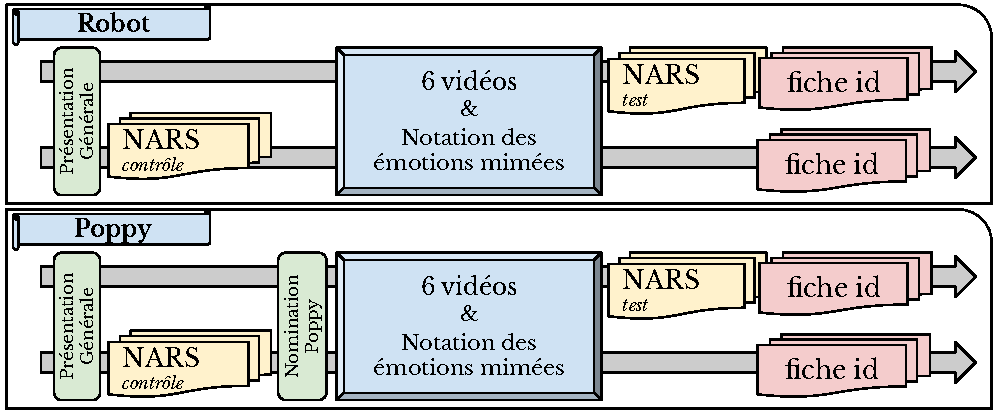
\includegraphics[width=\linewidth]{Figures/Desprez-proto-name_for_bot.pdf}
                    \caption{Protocole: \cro{un nom pour un robot}}\label{fig:proto-name_for_bot}
                \end{figure}
        \paragraph{Méthode} 
            Pour effectuer les passations, nous avons opté pour un formulaire en-ligne permettant ainsi une large diffusion ($N=106$), mais aussi par ce que le format vidéo imposait un support multimédia. 
            Les sujets étaient invités à visionner les vidéos (proposées dans un ordre aléatoire). Ces vidéos devaient être notées selon 6 critères émotionnels sur une échelle de -3 à +3 (de \gui{n'exprime absolument pas} à \gui{exprime parfaitement} telle émotion). Les 6 émotions sont le dégoût, la surprise, la joie, la colère, la tristesse et la peur.
            Deux conditions ont été créées, l’une où la question, portant sur la reconnaissance des émotions, était de la forme \gui{Poppy exprime\dots} et l’autre de la forme \gui{le Robot exprime\dots}. Parmi ces conditions, environ 20\prc des sujets effectuaient en premier lieu, la passation du \sht{NARS} pour constituer une ligne de base.
            \subparagraph{Matériel}
                \begin{figure}[!h]
                \begin{minipage}{0.375\linewidth}
                      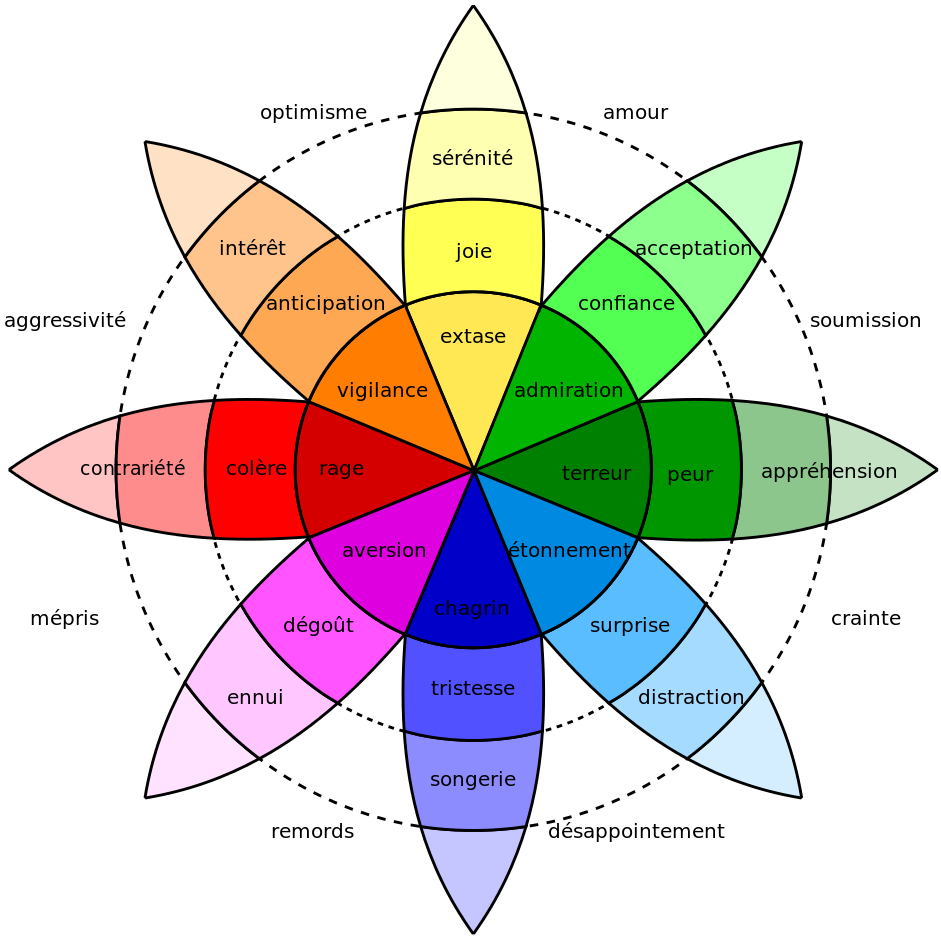
\includegraphics[width=\linewidth]{Figures/EmoModel.png}
                      \caption{Roue des émotions, Plutchik~\citeB{plutchik1991emotions}}\label{fig:EmoModel}
                \end{minipage}
                \hfill
                \begin{minipage}{0.6\linewidth}
                \myDefautStyle
                \subparagraph{Matériel vidéo}
                    Nous avons, dans certains cas, pu justifier clairement nos choix de mouvements, et dans d’autres nous avons dû nous baser essentiellement sur notre ressenti à l’aide de nos propres corps et en mimant les émotions nous mêmes ou encore en analysant certains cours de théâtre disponibles sur internet. Les archives de ces vidéos sont disponibles à une adresse \cro{non-répertoriée} permettant leur réutilisation future par d'autres équipes de recherche~\citeURL{TD-emo}.\newline\vfill
                \end{minipage}
                \end{figure}\par%
                \begin{itemize}\myItemStyle
                    \item    La tristesse: met en scène les mouvements classiques de la \gui{tragédie grecque} où l’homme se penche, prenant sa tête dans les mains pour pleurer.
                    \item    Le dégoût: l’idée était ici de mettre en scène l’apparition d’une odeur désagréable, le robot met une main sur son ventre, l’autre bouge légèrement devant son \gui{nez}.
                    \item    La joie: la difficulté d’exprimer la joie, sans l’aide du visage et avec une position des mains fixe (ouverte), était grande. L’idée était ici, d’avoir une sorte de danse de la victoire comme on peut l’observer dans certaines rencontres sportives.
                    \item    La colère: pour les mêmes raisons que la joie, cette expression était difficile à réaliser, pourtant le résultat est plutôt concluant.
                    \item    La surprise: certainement l’une des plus simple à réaliser, ici Poppy tourne la tête vers un objet qui le fait sursauter.
                    \item    La peur: est certainement la plus significative, car elle englobe l’émotion de la surprise tout en y ajoutant une notion de danger, caractérisée par la protection immédiate du corps (et principalement du visage) par les mains, puis par un moment d’attente et enfin de relâchement.
                \end{itemize}\par%
                Le score de reconnaissance:
                Pour chaque vidéo, on soustrait à la bonne réponse, la valeur moyenne des 5 mauvaises réponses. Exemple: vidéo colère: points colère - (moyenne (points: joie, tristesse, peur, dégoût, surprise).
                Puis on calcule la moyenne pour toutes les vidéos.\par%
                \vspace{-0.35cm}
                \begin{equation*}
                    Score=moyenne(V_T-(moyenne(V_n,V_n,V_n,V_n,V_n))
                \end{equation*}
                \newline\vspace{-1.75cm}
                \begin{multline*}\setstretch{1,0}\small
                    S=moy((V_1-(moy(V_2,V_3,V_4,V_5,V_6)));\\(V_2-(moy(V_1,V_3,V_4,V_5,V_6)));\dots\\\dots(V_6-(moy(V_1,V_2,V_3,V_4,V_5))))
                \end{multline*}
                \strut\hfill Score maximal: $S=5$ avec $V_n=0$ et $V_T=5$ \hfill Score minimal: $S=-5$ avec $V_n=5$ et $V_T=0$ \hfill\strut
        \paragraph{Résultats}
            \begin{figure}[!h]
            \begin{minipage}{0.425\linewidth}
                \centering
                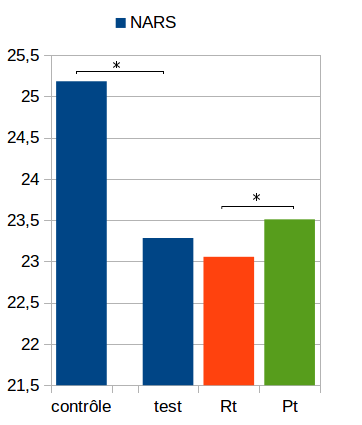
\includegraphics[width=.9\linewidth]{Figures/Desprez-nars-name_for_bot.png}
                \subcaption{Score obtenu au NARS}
                \label{fig:result-nars-name_for_bot}
            \end{minipage}
            \begin{minipage}{0.55\linewidth}
                \centering
                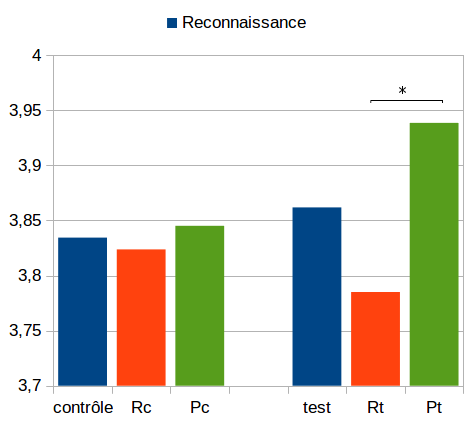
\includegraphics[width=.9\linewidth]{Figures/Desprez-BR-name_for_bot.png}
                \subcaption{Score de reconnaissance des émotions mimées}
                \label{fig:result-br-name_for_bot}
            \end{minipage}
            \caption{Résultats: \cro{un nom pour un robot}}
            \label{fig:result-name_for_bot}
            \end{figure}\par%
            Par rapport à nos hypothèses initiales, nous observons que, effectivement, nommer le robot par son prénom dans la formulation du questionnaire a un impact positif sur la capacité du sujet à déterminer la bonne émotion mimée dans les vidéos. En effet, sur la figure~\ref{fig:result-br-name_for_bot} nous voyons que dans la version \cro{test} (\sht{NARS} placé en aval) de la condition \cro{Poppy}, ici identifiée sous l'appellation \textit{Pt}, le score de reconnaissance est supérieur à 3,9~/~5, alors que dans le groupe \textit{Rt} ce score ne dépasse pas les 3,8~/~5. Bien que relativement faible, cette différence se révèle être significative par un test de Studente ($p=$). Notre 1\iere hypothèse est donc validée. \par%
            En revanche, pour la 2\nde, nous constatons sur la figure~\ref{fig:result-nars-name_for_bot}, un effet inverse à nos prévisions. En effet, les sujets de la condition \textit{Pt} obtiennent un score au \sht{NARS} plus élevé: 23,5 contre 23,05. Ici encore, bien que faible, cette différence se révèle être significative par un test de Studente ($p=$). Notre 2\nde hypothèse est donc \cro{inversement} validée, au sens où, la relation attendue fut observée mais avec des valeurs inverses.\par%
            Cette recherche, exploratoire, nous a permis d'observer deux autres effets inattendus: \Li la passation du \sht{NARS} en amont des vidéos biaise la reconnaissance. En effet, sur la figure~\ref{fig:result-br-name_for_bot}, nous constatons que l'effet observé en version \cro{test} (validant notre 1\iere hypothèse) disparaît totalement en version \cro{contrôle}. \ii le score initial au \sht{NARS} (groupe \cro{contrôle}, figure~\ref{fig:result-nars-name_for_bot}) est significativement plus élevé que pour le groupe ayant complété le questionnaire après le visionnage des vidéos: 25,2 contre 23,3 ($p=$).
        \paragraph{Conclusion}
            Ces résultats tendent à montrer que la nomination du robot est un facteur non négligeable, car elle impacte les perceptions de l'individu, et donc influencera l'interaction future. En effet, nommer le robot a permis une meilleure reconnaissance des sets de 6 émotions humaines qu'il mimait en vidéo. De plus, nous constatons que visionner ces vidéos diminue le score au \sht{NARS} comme si celles-ci avaient un pouvoir de sensibilisation, ou d'accommodation des sujets à la robotique. En revanche, si nous nous focalisons uniquement sur les résultats post-vidéos, on note que c'est dans la condition où le robot est nommé que le score est le plus élevé. Les raisons de cette diminution plus faible dans cette condition reste une question ouverte, tout comme les raisons pour lesquelles le \sht{NARS} placé en amont des vidéos biaise la reconnaissance.
    \subsection{Synthèse}
        Ainsi, cette double approche: longitudinale et ponctuelle, nous a permis d'enrichir nos connaissances sur les facteurs facilitant l'acceptabilité de la robotique. 
        Tout d'abord, \sht{EURO382} nous a permis de constater une évolution positive dans la perception de la robotique entre 2012 et 2017. Mais également de constater que les activités robotiques pratiquées par les élèves \tiret{et les différentes caractéristiques de celles-ci} influençaient cette dimension.
        Pour autant, nous n'avons pas été en mesure d'isoler, à posteriori, quelles caractéristiques mises en place par l'enseignant, avaient pu être déterminantes dans l'impact global observé. 
        Dans la seconde expérience présentée, nous avons pu mettre en lumière que ces caractéristiques déterminantes pouvaient se situer sur des éléments semblant insignifiants telle que la nomination de l'objet robotique qui, ici, a montré son impact sur la perception de l'objet en lui-même et des robots en général. % acceptabilité
%PART_3_CHAP_3_SEC_3
%WAIT a Review, ok
\clearpage
\section{Motivation}\label{chap:3.2}
    \subsection{Introduction}
        Pour cette thématique de la motivation, trois expérimentations sont ici présentées. La 1\iere est une proto-étude qui n'a jamais donné lieu à des passations expérimentales à proprement parler, mais qui a fourni plusieurs pistes de recherche et prétexté la construction de plusieurs ressources méritant d'être mentionnées. L'expérimentation suivante met en jeu le robot Poppy Dragster et sa notice de montage: ce robot développé dans l'optique de constituer une activité en soi pour le robot Ergojr, comme dérivation de celui-ci, donne une autre dimension à sa notice de montage qui devient alors une ressource pédagogique à part entière. Deux versions de cette notice ont été produites et sont ici comparées, notamment en terme d'efficacité dans la réalisation de la tâche mais aussi sur la perception par l'élève de la controlabilité de la tâche grâce au questionnaire \sht{IMI}. Enfin, la 3\ieme expérience propose d'étudier l'impact de la formulation des ressources pédagogiques sur, d'une part, la difficulté perçue (également via le \sht{IMI}) et, d'autre part, sur la compréhension des notions abordées dans l'activité. Mais, cette seconde sera abordée en section suivante~\citeS{chap:3.3}.
    \subsection{Proto-expérience}
        %\paragraph{\textit{Exp}: \cro{les a-priorie en robotique}}\label{Exp:a_priorie}
            %Il s'agit d'évaluer ici l'envie et la difficulté perçue par l'apprenant à réaliser une activité robotique. Deux contexte: les élèves entrent dans la salle de \sht{TD} où le matériel est pré-positionné; \Li présenter l'activité dans le détail et répondre à toutes les questions qui seront posées, ou \ii ne rien faire. Puis demander à l'apprenant d'estimer la difficulté de la tâche en fonction de ses capacités~\citeB{bandura1986explanatory} \ie \cro{vous vous sentez capable d'accomplir cette tâche} oui/non; puis d'estimer le degré de certitude de sa réponse (via une échelle likert) et de même sur son envie~\citeB{atkinson1957motivational}. Faire réaliser l'activité. Enfin, demander s'il pense avoir réussi l'activité et pourquoi~\citeB{weiner1985attributional}. Ce type de protocole peut être intégrater avec de multiple types de d'activité. 
        \paragraph{\textit{Exp}: \cro{Rôle du support}}\label{Exp:Role_support}
            Ici, l'objectif de ce protocole est de mettre en évidence les difficultés de gestion des différents supports durant l'activité et les effets de double tâche induits par cela~\citeS{sec:double-tache}.
            Ici, la même activité (\eg thème, question posée, information donnée, \etc) est proposée au sujet selon quatre formats: \Li un support \sht{pdf} présenté numériquement, \ii présenté en version papier, \iii adapté en vidéo et \iiii intégré directement dans l'interface de programmation (dans notre contexte \sht{snap}). L'hypothèse serait que le \Li n'offrirait aucun avantage face à sa version papier, comme ce que nous avons constaté~\citeS{sec:support}. En revanche, les difficultés d'utilisation d'un même écran \tiret{alternant interface de programmation et ressources vidéos} ne garantissent pas son avantage sur les ressources papiers. De même, le format intégré, et la perte de contrôle qu'il implique~\citeS{sec:contro} ne garantissent pas son avantage sur un format vidéo ou même papier.
            \subparagraph{Matériels vidéo}
                À ces fins, 3 vidéos ont été réalisées~\citeURL{TD-chicken-td} et les premières ébauches de l'activité \cro{poule}~\citeS{sec:act_poule} et de la démo \cro{têtu} ont été créées.
                La vidéo1 présente l'environnement \sht{snap}: comment créer une variable et la modifier. Elle montre ensuite comment accéder à une catégorie et déplacer un bloc. Ainsi, 2 blocs sont alors posés sur la zone de script: 'set position' et 'all motors' permettant respectivement de déplacer un moteur dans une position; et de récupérer le nom des moteurs du robot. Puis elle réutilise la variable créée ultérieurement, en l'insérant dans le bloc \cro{set position}, elle correspond ainsi à la valeur en degrés de la position à atteindre. Enfin, elle montre comment attribuer une variable à chacun des 3 moteurs de la base du robot et introduit le bloc 'forever' (pour toujours); ce petit code permet ainsi de déplacer le robot réel et virtuel grâce à la manipulation des variables. Quatre notions sont ici développées: créer/modifier une variable; répartition des blocs en catégories; contrôler le robot; la boucle 'forever'
                Ils sont alors invités à réaliser eux-mêmes ce qu'ils viennent de voir et à faire leurs propres tests. C'est à ce moment qu'ils commencent à coder et manipuler le robot. Quinze minutes après le début de l'activité ils sont invités à regarder la deuxième vidéo.\par%
                La vidéo2 présente un algorithme à réaliser: le \cro{comportement poule}. L'objectif est de contrôler les 3 moteurs supérieurs (m4, m5, m6) via les 3 moteurs de la base (m1, m2, m3), pour qu'ils compensent leurs mouvements (exemple: si m1=+30° alors m4=-30°). La première étape présente comment simplifier (optimiser/factoriser) les écritures en utilisant les listes. Puis, est montré comment associer les moteurs entre eux (assemblage de plusieurs blocs). Enfin comment (via le bloc 'map') inverser la valeur des positions des moteurs de la base. Pour terminer, une démonstration de l'exécution du programme sur le robot réel et sur le robot virtuel est fournie. Trois notions sont ici développées: créer/modifier une liste; récupérer les informations des senseurs du robot; consolider les manipulations précédentes.\par%
                30 min plus tard, la vidéo3 propose un défi: réaliser le \cro{comportement têtu}. Elle commence par une démonstration du comportement sur le robot réel. Puis elle fournit l'algorithme qui produit ce comportement: \gui{je me souviens de ma position de départ. Pour toujours, si j'ai bougé: alors, je retourne dans ma position de départ, sinon, j'attends 1 seconde.} Un certain nombre d'indices/astuces sont fournis jusqu'à la fin de la vidéo pour réussir à coder ce comportement en moins de 45min.
            \subparagraph{Limite}    
                Cependant, la difficulté de produire des vidéos évoluant aussi rapidement que le matériel \sht{pdf} nous a empêché de mener à bien ce type d'expérience. De plus, il en est de même pour les supports intégrés qui \tiret{pour permettre une ergonomie de mise à jour suffisante} auraient nécessité un investissement trop grand. En revanche, un didacticiel directement intégré à \sht{snap} a été réalisé dans ce sens, mais n'a pas donné suite. Il est aujourd'hui toujours disponible en ligne~\citeURL{TD-discover-td}, il se compose d'une phase interactive de découverte (environ 45min) puis d'une phase pratique de programmation où l'utilisateur applique les notions abordées précédemment, puis après un temps défini (45 min par défaut), une série de comportement est présentée et explicitée pendant environ 30min (phase passive). Dans sa forme actuelle, ce didacticiel est trop \cro{riche} d'informations pour permettre leur bonne assimilation; cependant, il offre un bon complément pour des personnes averties. 
    %dragster
    \subsection{\textit{Exp}: \cro{Notice modulaire ou linéaire} }\label{Exp:dragster}
        \myPhantom{paragraph}{Introduction}
            Nous voulons évaluer ici la perception de la contrôlabilité~\citeS{sec:viau} des étudiants et voir l’impact des différentes pratiques d’activités sur leur apprentissage, leur satisfaction et leur perception des tâches.
            La perception de la contrôlabilité correspond au niveau de contrôle que les étudiants pensent avoir sur la réalisation de l'activité et de ses résultats. Cela peut être créé en responsabilisant les étudiants, en les laissant faire des choix. Nous voulons donc avoir un groupe qui fera des choix entre plusieurs options proposées, tandis que l’autre groupe devra suivre les instructions pas à pas.
            L’autorité et le monopole du professeur peuvent faire tomber ce sentiment de choix, c’est pourquoi nous devrions intervenir le moins possible avec le groupe sauf si cela est nécessaire, ne pas leur donner des instructions autoritaires et les laisser prendre leurs décisions jusqu’à ce qu’ils nous appellent pour validation. Notre objectif est de concevoir des activités d’assemblage pouvant être présentées sous un format linéaire (instructions à suivre pas à pas) ou sous un format modulaire (différentes feuilles à choisir).
        \paragraph{Méthode}
            Étant donné que c’est la première fois que le robot Dragster est présenté et utilisé par les étudiants, nous souhaitons mettre l’accent sur l’assemblage plutôt que sur les activités de programmation. Les activités de programmation seront les mêmes pour les deux groupes, l’assemblage sera différent. C'est pourquoi les étudiants seront répartis en deux groupes, chaque groupe se trouvant dans une pièce différente.
            \subparagraph{Population}
                Les sujets venaient visiter le centre Inria Sud-Ouest, ils étaient donc disponibles le matin pour l'expérience. Comme ils avaient tous moins de 18 ans ($\overline{x}=$16~ans), un formulaire de consentement signé par les parents était obligatoire~\citeS{sec:adm}.
                Il y avait 35 étudiants: 12 filles et 18 garçons, de 1\iere S3 lycée La Sauque, ils ont été divisés en 2 groupes: \sbg{GM}, 15 étudiants (5 groupes de 3); \sbg{GL}, 15 étudiants (5 groupes de 3); 5 autres étaient dans un groupe qui n'a pas participé à l'étude.
            \subparagraph{Hypothèses}
                Selon le modèle Viau de motivation de l'étudiant, les étudiants peuvent influencer positivement leurs progrès sur l'activité par leurs choix, en se sentant responsables et en contrôle. Ainsi, le groupe avec l'assemblage présenté dans un format modulaire (GM) devrait se sentir plus en contrôle avec un sentiment de choix plus élevé et avoir plus de progrès dans l'activité d'assemblage.
                Ainsi, nos hypothèses sont que le groupe \sht{GM} sera plus satisfait (plus de plaisir et plus de choix) et plus efficace (moins d'effort et plus rapide) en ce qui concerne la réalisation de la tâche en raison de la liberté de choix induite par les différents modules.
            \subparagraph{Matériel}
                Guide de montage et de configuration \sht{GL}~\citeA{pdf:notice_dragster_lin}, le tout dans une feuille continue. La fiche d'activité est remise aux étudiants avec les pages jointes. Ils suivent donc les tâches une à une (assemblage électronique, configuration du moteur, assemblage mécanique de la base puis du bras, test du robot) selon l'ordre imposé.
                Guide de montage et de configuration \sht{GL}~\citeA{pdf:notice_dragster_mod}, séparé en 8 feuilles différentes. Les instructions sont écrites sous la forme passive pour donner la liberté dans les actions au lieu de donner des instructions (par exemple: \cro{les moteurs peuvent être configurés en entrant cette commande} au lieu de \cro{définir les moteurs avec cette commande}). Les étudiants peuvent choisir la feuille de départ même s'il y a des actions à faire avant d'autres (le test ne peut pas être effectué si les moteurs ne sont pas configurés). Si ce cas arrive, les étudiants doivent se rendre compte qu'ils doivent effectuer des tâches préliminaires.\\
                \begin{figure}[!h]
                    \centering\label{fig:drag_proto}
                    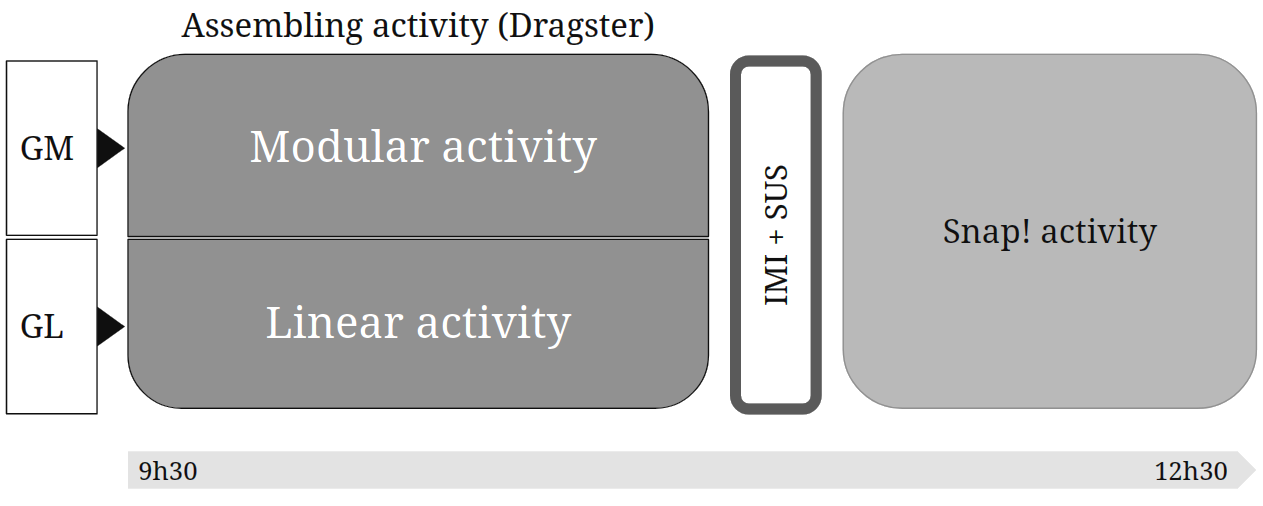
\includegraphics[width=0.9\linewidth]{Figures/Gilliard-proto.png}
                    \caption{Protocole: \cro{Notice modulaire ou linéaire}}
                \end{figure}
                Une même activité a été proposée après le montage du robot~\citeA{pdf:act_dragster}. Elle permettait, entre autres, de remarquer et de corriger les erreurs potentielles lors du montage. L'activité explorait les fonctions de base telles que le déplacement d'un moteur, puis un peu plus complexes avec de la détection d'objets basée sur la boucle sensori-motrice.\par%
                Entre le montage et l'activité, deux questionnaires individuels ont été complétés par les étudiants: le \sht{SUS}~\citeS{q:sus} et 4 sous-échelles du \sht{IMI}: Intérêt~/~plaisir, Compétence perçue, Effort~/~Importance, Choix perçu~\citeS{q:imi}. Les réponses recueillies sur papier ont été extraites avec \sht{amc}. Un test de Student unilatéral pour deux échantillons à variance inégale est utilisé pour estimer la significativité des résultats.\par%
                L'expérimentation (accueil et répartition des groupes / montage du dragster / questionnaires / activités) se déroula sur une matinée entière: de 9h30 à 12h30.
                Au préalable, une étude pilote sur 3 étudiants de 22 ans (qui n’avaient jamais programmé auparavant) a été réalisée afin de détecter les erreurs potentielles dans les fiches d’activités, les images ou informations manquantes et également de vérifier l'estimation du temps de construction du dragster. Les résultats et les retours d'expérience de l'étude pilote nous ont aidés à clarifier des parties importantes et à confirmer la validité des activités.
        \paragraph{Résultats}
            Suite à l'expérimentation, nous observons~\citeF{fig:result_dragster} que, concernant l’assemblage, il existe une différence significative (test de Student, $p=1.88e-10$) entre \sht{GM} ($\overline{x}=62$ minutes). et \sht{GL} ($\overline{x}=109$ minutes). Pour le test \sht{IMI}, les résultats montrent qu'il existe une différence significative positive pour \sht{GL} avec l'échelle \cro{choix} ($p=0,04287$). Nous  notons, qu'il n’y a aucune différence entre les groupes pour les autres échelles \sht{IMI} \cro{compétence} ($p=0,37849$), \cro{plaisir} ($p=0,39675$) et \cro{effort} ($p=0,21155$); ni pour le SUS ($p=0.24412$).
            \begin{figure}[!h]
                \centering
                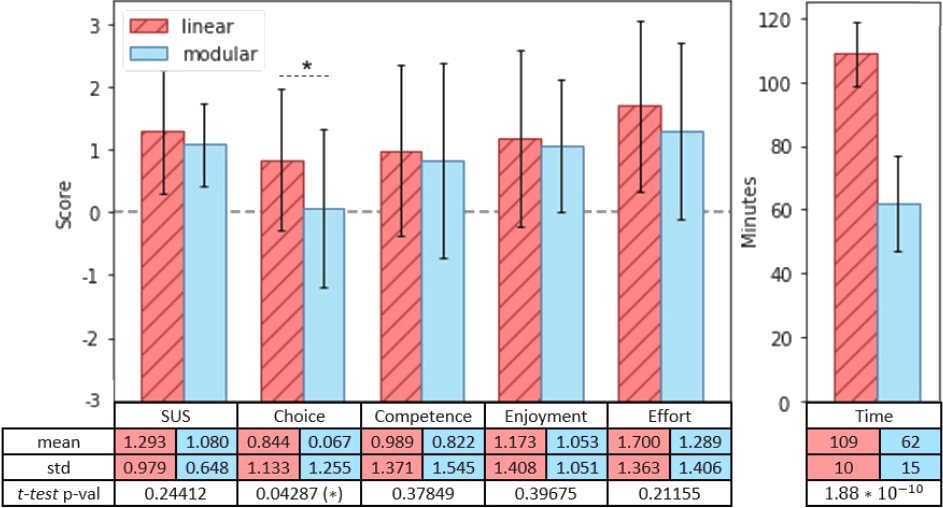
\includegraphics[width=0.9\linewidth]{Figures/Gilliard-result}
                \caption{Résultats, \cro{Notice modulaire ou linéaire}}
                \label{fig:result_dragster}
            \end{figure}
        \paragraph{Conclusion}
            %les résultats ont montré que la contrôlabilité et le choix dans une activité modulaire placeraient les étudiants dans une attitude plus \cro{active}, même s'ils ont le sentiment d'avoir eut moins de choix
            Le groupe \sht{GM} était presque deux fois plus rapide que le groupe \sht{GL}. Cela pourrait s'expliquer par le fait que la tâche d'assemblage était plus facile à répartir entre les trois membres de chaque groupe en raison des feuilles séparées (par exemple, on peut assembler des roues tout en assemblant des bras). Dans les observations, presque tous les groupes \sht{GM} se sont divisés en tâches tandis que dans le groupe \sht{GL} certains membres étaient totalement passifs. Ainsi, notre hypothèse sur le temps d'assemblage qui diffère entre les groupes est acceptée.
            sur les aspects motivationnels, nous nous attendions à un sentiment plus important de liberté de choix dans le groupe \sht{GM} en raison de la possibilité de choisir entre les feuilles et le vocabulaire utilisé (suggestions et non ordres). 
            Cependant, l’échelle \cro{Choix} est significative mais est à l’inverse de ce que nous avions prédit: le sentiment de choix est plus élevé pour le groupe \sht{GL}. Ainsi, notre hypothèse sur le sentiment de choix plus élevé pour le groupe \sht{GM} est rejetée. Ce résultat pourrait être dû au fait que les organisations internes de chaque groupe d'élèves fait émerger une forme de leadership qui pourrait induire une forme de contrainte au sein des groupes et réduire le sentiment de choix.
    %poule
    \subsection{\textit{Exp}: \cro{Décrire ou manipuler}}\label{Exp:poule}
        \myPhantom{paragraph}{Introduction}
            Nous voulons ici évaluer l’impact de la manipulation tangible~\citeS{sec:tangible}  sur les étudiants. Une manipulation tangible peut créer une immersion dans l'expérience. Il peut soutenir la cognition spatiale des utilisateurs, réduire la charge cognitive et permettre une immersion plus créative dans le problème. Cela peut également donner plus d'autonomie à l'apprenant, lui permettant de corriger ses erreurs et de comprendre les concepts abstraits qui se cachent derrière. Il est déjà apparu comme un support efficace pour la programmation. En plus d’avoir accès en classe à leur robot, nous souhaitons que les étudiants profitent des possibilités de manipulation: le robot n’est ni fragile, ni dangereux, ni simple à manipuler. Nous voulons les amener à être plus actifs dans la manipulation et à tester si cela affecte leur perception de l'activité et les résultats du quiz.
        \paragraph{Méthode}
            Nous avons décidé de créer deux situations d'apprentissage: l'une axée sur la démonstration (l'étudiant doit reproduire l'action présentée), l'autre sur la description (l'étudiant doit reproduire l'action décrite). Nous voulions une action simple impliquant des boucles sensori-motrices afin que les étudiants puissent manipuler leur robot avec leurs mains et avoir un retour direct. Un \cro{comportement animal} semblait adapté et intéressant à recréer.
            Pour ce faire, nous présentons à chaque groupe une activité de quatre pages~\citeA{pdf:act_poule}. Seule la dernière page diffère des autres en fonction de \cro{Description} ou \cro{Démonstration}~\citeF{fig:act_poule}. Ils doivent reproduire le mouvement d'une \cro{poule} (la tête du robot reste stable lorsque son corps est déplacé), soit en observant et en manipulant son robot, soit en suivant une liste de conseils pour créer le comportement souhaité. Avant de commencer la dernière page, une vidéo du comportement d'une poule~\citeURL{TD-chicken-move}  est affichée.
            \subparagraph{Population}
                Les sujets étaient des lycéens de lycées en partenariat avec Inria~\citeS{sec:etablisements}.
                Il y avait 66 étudiants du lycée St Genes et du lycée Condorcet. 14 élèves ont été retirés parce qu'ils n'avaient pas terminé l'activité évaluée ou n'avaient complété l'ensemble des pages des questionnaires; 24 étaient des filles, 28 des garçons, d'une moyenne d'âge de 15 ans. À chaque intervention, le groupe d'élève était divisé en deux groupes: \sht{GDemo} et \sht{GDesc}. Les 54 étudiants formaient un ensemble hétérogène: certains étaient issus de filière \cro{scientifique}, d'autres de filière \cro{littéraire} mais aucun n'avait effectué d'activité robotique en classe.
            \subparagraph{Matériel}
                L'activité proposée possédait deux variantes~\citeS{sec:act_poule}. En fin d'activité, chaque étudiant complétait un quiz composé de 6 questions portant sur les notions abordées dans l'activité~\citeA{pdf:qcm_poule}; puis il complétait 4 sous-échelles du \sht{IMI}: Intérêt~/~plaisir, Compétence perçue, Effort~/~Importance, Pression~/~tension~\citeS{q:imi}.
            \subparagraph{Hypothèse}
                La manipulation tangible peut conduire à une plus grande immersion dans le problème et peut donner plus d'autonomie à l'apprenant, permettant de corriger soi-même les erreurs et de comprendre les concepts plus précisément~\citeS{sec:tangible}. Pour nos hypothèses, nous nous attendons à ce que la manipulation tangible ait un impact plus fort sur les résultats d'apprentissage évalués par le quiz du groupe de démonstration. Les autres échelles du \sht{IMI} sont utilisées à titre exploratoire et pourraient nous aider à mieux interpréter les résultats.
            \subparagraph{Déroulement}
                Tous les étudiants arrivent en classe en même temps et sont assis par groupes de deux étudiants par table et avec un ordinateur et un kit robotique.
                Qu'ils soient dans le groupe \cro{Description} ou \cro{Démonstration}, ils font tous, les trois premières feuilles d'exercices à la vitesse qu'ils désirent. Nous leur donnons les feuilles une par une. Ils doivent donc nous appeler quand ils ont terminé avec une feuille pour obtenir la suivante. Avant de leur donner la feuille suivante, nous effectuons une rapide vérification avant qu’ils ne continuent. Comme les premières feuilles sont plus faciles que la quatrième, ils sont assez autonomes dans leur travail. Ils sont autorisés à parler avec leur partenaire, cependant, ils ne doivent pas communiquer avec d'autres groupes. 
                Finalement, quand ils ont fini avec la troisième feuille, ils commencent le \cro{défi poule} qui est la partie qui nous intéresse. Ils regardent la vidéo de démonstration et commencent à créer leurs fonctions avec \sht{snap}. 1h50 après leur entrée en classe, par contrainte de temps, ils doivent s'arrêter là où ils sont et remplir le quiz puis le questionnaire. Une fois qu'ils ont terminé, ils peuvent quitter la classe.
                Les réponses collectées sont extraites avec \sht{amc} et converties en fichiers csv. Un test de Student unilatéral pour deux échantillons à variance inégale est utilisé pour estimer la significativité des résultats.\par%
                Nous avons organisé 6 sessions de notre expérience, toutes entre mai et juin. Au préalable, nous avions effectué une étude pilote sur 5 lycéens (1 groupe de 3 et 1 groupe de 2) avec ErgoJr au centre Inria avant de faire des expériences en classe. Cela nous a permis d'ajuster et de clarifier certaines instructions. Nous avons également rencontré les enseignants et visité les deux salles de classe une semaine avant pour vérifier l’ordinateur, la connectivité et les détails techniques afin de s’assurer que tout fonctionne directement le jour des expériences.
        \paragraph{Résultats}
            Pour le groupe \sht{GDemo} la perception de la quantité d'effort à fournir pour réaliser l'activité est plus faible que pour le groupe \sht{GDesc} ($p=0.042$) et ils obtiennent un score plus élevé au quiz ($p=0,067$). Nous observons également que les échelles de compétence, d’effort, d’intérêt et de quiz sont positives pour les deux groupes, tandis que l’échelle de pression est négative. Cependant, les échelles Compétence, Intérêt et Pression ne sont pas significativement différentes entre ces deux groupes.
            Les résultats concernant le quiz sont détaillés dans la section suivante~\citeS{Exp:poule_2}
            \begin{figure}[!h]
                \centering
                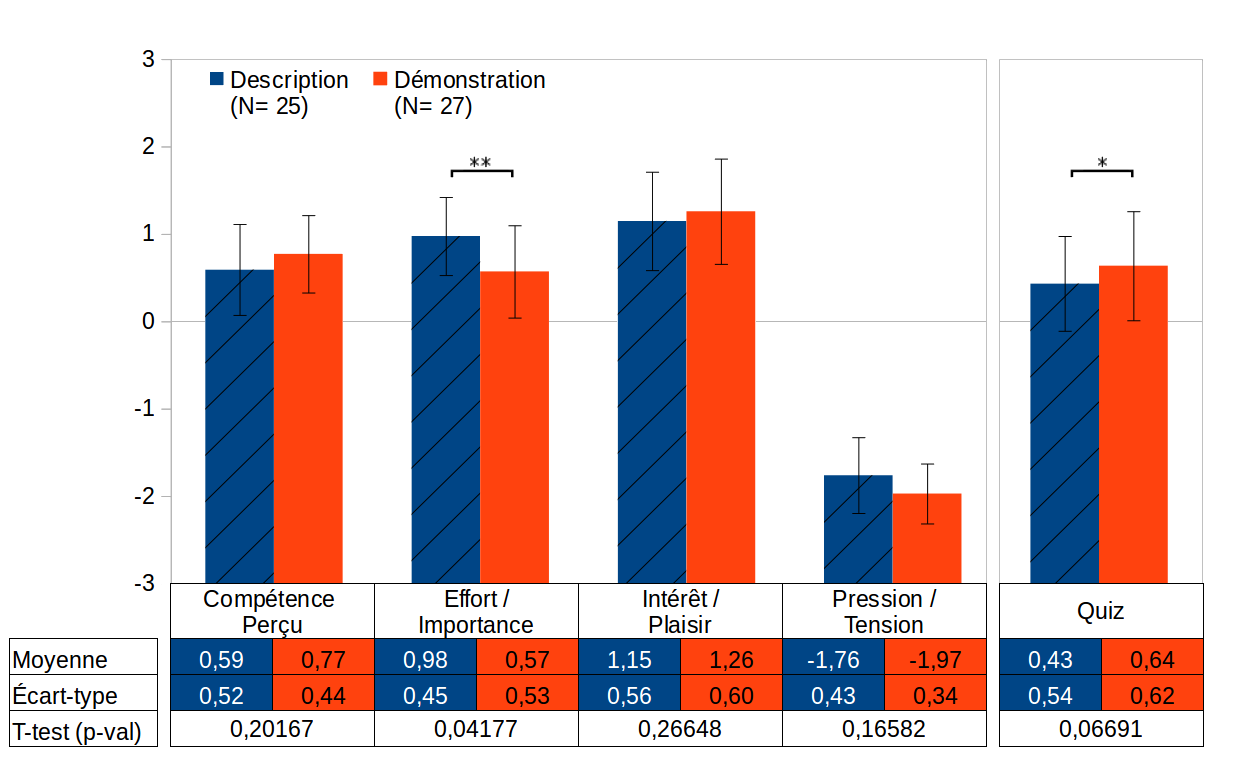
\includegraphics[width=0.9\linewidth]{Figures/Desprez-result_poule.png}
                \caption{Résultats globaux \cro{Décrire ou manipuler}}\label{fig:result_poule}
            \end{figure}
        \paragraph{Conclusion}  
            L’étude a été répliquée dans 6 contextes différents, à chaque fois, le groupe d'élèves fut réparti entre les deux conditions \sht{GDemo} et \sht{GDesc}. Même si les groupes sont hétérogènes, cela permet d’avoir une étude beaucoup plus réaliste et écologique qui s’adapte à la variabilité naturelle de notre population de \gui{lycéens} (variant entre deux lycées avec des étudiants de différents parcours, origines, motivations, \etc). Nous constatons qu'une activité mettant en jeu une démonstration tangible des objectifs à atteindre permet de réduire l'effort perçu par l'élève et potentiellement de lui offrir de meilleurs résultats en terme d'acquisition de connaissances.
    \subsection{Synthèse}
        Les expériences ici menées ne nous permettent pas d'observer si il existe un avantage à exercer une activité robotique (en matière de gain motivationnel) comparé à une activité lambda. Cependant, on note que \Li l'obligation de telles pratiques (via les programmes officiels) rend cette distinction peu pertinente (les deux types d'activités devant être réalisés pour d'autres raisons que le seul aspect motivationnel); et que \ii la proximité d'aujourd'hui entre technologie robotique et nouvelles technologies rend les résultats, qui seraient obtenus pour cette distinction, peu pérennes.
        Ainsi, nous avons choisi d'aborder les caractéristiques de mise en place des activités robotiques et leurs impacts motivationnels relevés ici via le questionnaire \sht{IMI}. Nous avons observé dans une première expérience que lors d'une tâche de construction d'un robot le sentiment de contrôle sur l'activité variait avec le format des ressources fournies (\eg modulaire \textit{vs} linéaire): l'activité modulaire, bien que, objectivement plus libre dans sa réalisation, a obtenu le sentiment de contrôle le plus faible. Dans une seconde, nous avons vu que dans le cadre d'un \sht{TD}, la formulation et les démonstrations fournies impactaient le sentiment d'effort: une démonstration tangible semble permettre une meilleure compréhension de l'objectif à atteindre et donc de l'effort à fournir pour sa réalisation; pour s'en assurer, il faut mesurer si les élèves ont objectivement mieux compris les concepts nécessaires à la réalisation de l'objectif.  % motivation
%PART_3_CHAP_3_SEC_4
%WAIT a Review, ok
\clearpage
\section{Connaissances}\label{chap:3.3}
    \subsection{Introduction}
        Pour cette dernière thématique, deux expérimentations sont présentées. La 1\iere correspondant à la seconde partie de l'expérience développée en section précédente~\citeS{Exp:poule}: ici, nous présentons les résultats obtenus au quiz qui étaient associés à l'activité. La 2\nde, exploitant l'activité \textit{danse}, se présente sous forme de deux déclinaisons: l'une étant une version exploratoire, l'autre étant une version plus aboutie et focalisée mais n'ayant pas encore été réalisée.
    %montrer / decrire
    \subsection{\textit{Exp}: \cro{Décrire ou manipuler}}\label{Exp:poule_2}
        \myPhantom{paragraph}{Introduction}
            Durant l'expérimentation décrite en section précédente~\citeS{Exp:poule}, nous avons, en plus des aspects motivationnels, évalué les connaissances misent en jeu durant l'activité.
        \paragraph{Résultats}
            Une première constatation est que globalement le \sht{GDemo} a mieux réussi le quiz tout en ayant l'impression de fournir moins d'efforts~\citeF{fig:result_poule}. 
            \begin{figure}[!h]
                \centering
                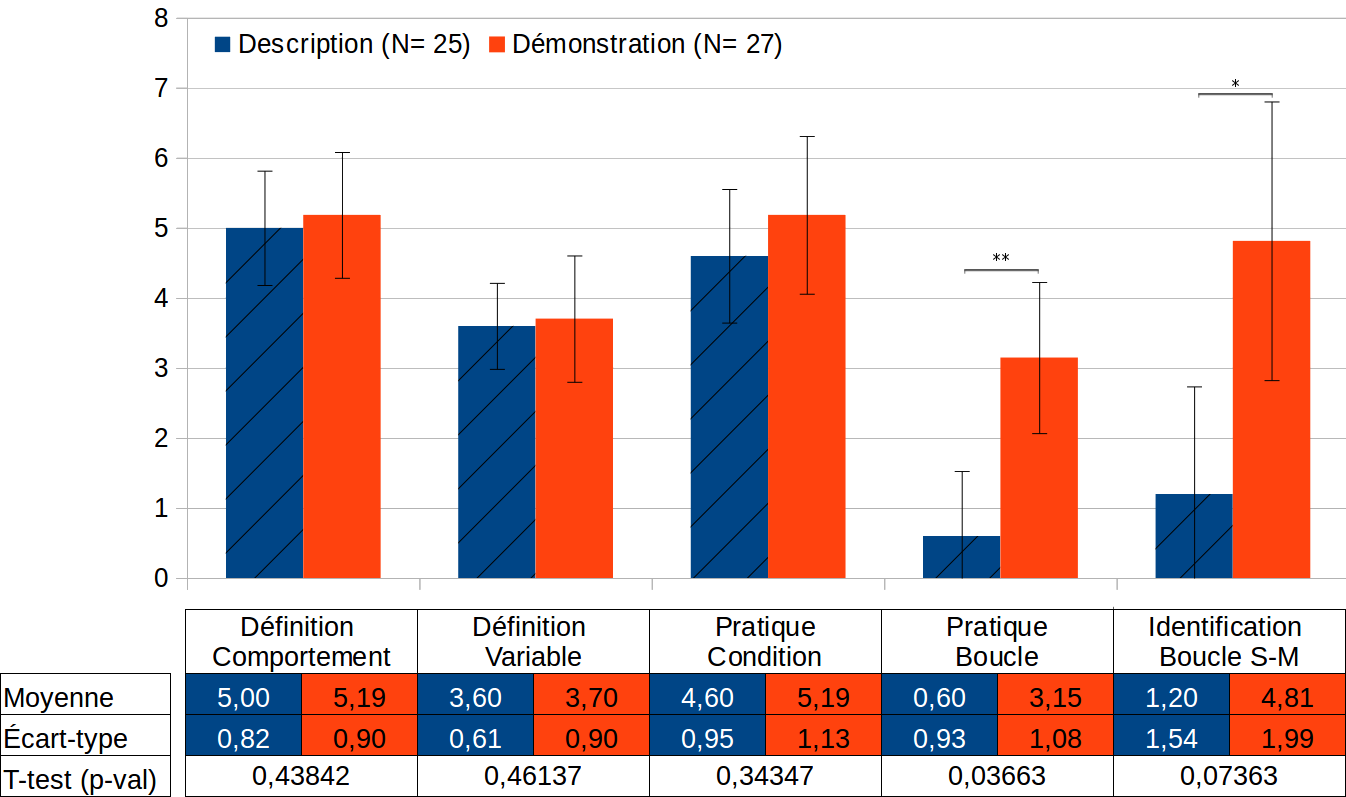
\includegraphics[width=0.9\linewidth]{Figures/Desprez-result_poule-quiz.png}\label{fig:result_poule-quiz}
                \caption{Résultats quiz: \cro{Décrire ou manipuler}}
            \end{figure}\par%
            Sur les cinq questions que comportait ce \sht{QCM}~\citeA{pdf:qcm_poule} seules les deux questions portant sur les boucles ont obtenu des résultats significativement moins bons en condition \sht{GDesc}.
            \begin{enumerate}\myItemStyle
                \item définition; \gui{Qu’appelle-t-on le comportement d’un robot?}
                \item définition; \gui{Qu’est ce qu’une variable?}
                \item illustration; \gui{\sht{snap} vous demande, si tous les moteurs doivent être mis en compliant}
                \item illustration; \gui{Que produisent ces instructions?}
                \item identification; \gui{Parmi ces 10 exemples, où y a t-il une ou plusieurs boucles sensori-motrices}
            \end{enumerate}{}
        \paragraph{Conclusion}
            Nous constatons donc que sur un temps court (sessions d'activités de moins de deux heures) la manipulation directe de la notion à intégrer, ici, la \bg{BSM} est plus favorable. En effet, cette configuration a permis aux élèves non seulement d'améliorer leurs performances au quiz final, mais aussi d'avoir la perception d'avoir fourni moins d'efforts~\citeS{Exp:poule}. Cependant, cette impression de \cro{moindre effort} peut être en décalage. En effet, l'objectif affiché est de réaliser le défi et de produire le comportement \cro{poule} or pour le \sht{GDemo}, cette production est déjà réalisée, pouvant ainsi donner l'illusion de la réussite. Mais, l'objectif pédagogique se trouve ailleurs: le but de cette activité de découverte est de permettre à l'élève d'appréhender et d'identifier une \sht{BSM}. Ainsi, cela a plusieurs avantages: le défi induit par la scénarisation permet d'engager les élèves ou, au moins, de les intriguer. Une fois dans l'activité, fournir une solution tangible permettant d'expérimenter le résultat attendu (ici, le comportement \cro{poule}) offre le double avantage de donner une impression de réussite aux élèves sur leurs objectifs directs (réussite au défi) et d'améliorer \tiret{du moins à court terme} leur compréhension du sujet abordé (ici, la \sht{BSM}. 
    %Reel_virtuel    
    \subsection{\textit{Exp}: \cro{Robot virtuel ou réel, danse avec un robot}}\label{Exp:Reel_virtuel}
        \myPhantom{paragraph}{Introduction}
            Au vu de la difficulté pour certains établissements scolaires de s'équiper en matériel robotique~\citeS{sec:materiel}, nous avons cherché à montrer dans cette expérimentation dans quelle mesure l'utilisation d'une version simulée en tant que substitut à un robot réel \tiret{perdant ainsi les avantages inhérents aux objets tangibles} pouvait avoir un intérêt suffisant. Pour aller plus loin, dans quelle mesure l'aspect tangible est prédominant pour l'apprentissage de la robotique? auquel cas, des ressources comme des \cro{activités débranchées\footnote{(activité en informatique, robotique, numérique, \etc, ne nécessitant pas de matériel informatique, typiquement un ordinateur}} pourraient s'avérer plus efficaces qu'une version simulée d'un robot.
        \subsubsection{Étude pilote}\label{Exp:Reel_virtuel-pilote}
            \paragraph{Méthode}
                Sur une unique session de 2 heures, les élèves ($n=30$) étaient répartis en 2 groupes~V et~R, l'un manipulant le visualisateur ($n=16$), l'autre manipulant le robot réel ($n=14$). L'objectif était d'évaluer la différence qui pourrait exister entre la manipulation d'un robot réel et un robot virtuel simulé.\\
                \sbg{VI}: 
                Quatre conditions: \Li robots réel+virtuel (RV), \ii uniquement la version réel (R), \iii uniquement la version virtuelle (V) et \iiii une activité de démonstration (AD) sans manipulation ni programmation du robot.\\
                \sbg{VD}: 
                \begin{itemize}\myItemStyle
                    \item Motivation, mesurée par questionnaires avant et après expérience
                    \item Connaissances acquises, mesurées par questionnaires après expérience
                    \item Satisfaction, mesurée par questionnaires après expérience
                    \item Réussite, mesure du niveau de progression dans l'activité
                \end{itemize}{}
                \subparagraph{Hypothèses}
                    D'un point vue général, nous pouvons émettre l'hypothèse (qui sera uniquement discutée ici) que la motivation sera maximale lorsque l'étudiant peut manipuler les versions réelles et virtuelles du robot; que la motivation lors de l'utilisation seule du robot réel reste supérieure à l'utilisation seule du visualisateur. Les trois précédentes seront supérieures à la simple démonstration passive des activités; ainsi pour la motivation: RV~>~R~>~V~>~AD.
                    De plus, augmenter la motivation \etou la satisfaction à utiliser un support pédagogique favorise l'acquisition des concepts véhiculés dans ce support; ainsi, nous pouvons supposer que pour la connaissance et la réussite: RV~>~R~>~V~>~AD, si pour la motivation: RV~>~R~>~V~>~AD. 
                    Enfin, nous pouvons émettre comme dernière hypothèse que ces relations seront exacerbées lorsque la satisfaction est positive.
                    Afin d'évaluer au mieux ces hypothèses, il a été décidé de diviser celles-ci en plusieurs sous groupes afin d'effectuer des études pilotes pour étalonner nos activités et nos questionnaires.
                    L'hypothèse intermédiaire (qui sera traitée ici) est que la motivation est supérieure avec le robot réel seul comparé au virtuel seul; ainsi, pour les quatre \sht{VD}:~R~>~V.
                \subparagraph{L'activité}
                    Elle est divisée en deux grandes parties, prise en main (\sht{snap} et robot) et un défi, cette activité propose un déroulement \cro{cadré}: présentation d'une notion/manipulation, exemple, mise en pratique, présentation d'une deuxième, \etc. Cette progression guidée est réalisée par l'élève grâce à un document papier qui lui est fourni~\citeA{pdf:act_dance} et dure entre 30 et 45min. Ensuite un défi est proposé: trouver les 6 paramètres moteurs (position en degrés) afin que le robot atteigne la position donnée dans une photo illustrative; le but étant de trouver un maximum de positions différentes (16 au total) en environ 1~heure.
                \subparagraph{Les questionnaires}
                    Ceux ici utilisés sont des compositions de différents questionnaires existants nous permettant une posture exploratoire quant aux résultats de cette étude pilote. Ainsi, un questionnaire évaluant leur motivation fut effectué avant~\citeA{pdf:qcm-pre_dance} et après l'activité par chaque élève. Des questions additionnelles ont été ajoutées aux questionnaires pré et post activité afin d'identifier chez les élèves leur profil, leur satisfaction et leurs connaissances acquises~\citeA{pdf:qcm-post_dance}. Plusieurs questions relatives aux différents concepts qui englobent la motivation ont donc été posées. Dix-huit éléments étaient communs au questionnaire pré et post-activité. Réparties en différentes catégories, elles évaluent: la motivation intrinsèque (4\sht{ques}) et extrinsèque (4\sht{ques}); l'autodétermination et l'auto-efficacité (6\sht{ques}); les facteurs environnementaux (4\sht{ques}). Ces 18 affirmations (9 positives, 9 négatives) étaient à évaluer suivant une échelle le Likert. Ce questionnaire a été construit suivant différents éléments de la littérature notamment le \sht{SUS} et les résultats de Kaloti-Halla~\citeB{kaloti2015students}.
                    En accord avec Harter~\citeB{harter1981new} cinq affirmations à compléter ont été ajoutées au questionnaire pré-activité pour tenter d'établir des profils d'apprenants. À chaque affirmation trois réponses étaient possibles et rapportaient de 0 à 2 points, déterminant ainsi un score sur~10. Trois profils ont été définis A~(>6), B et C~(<=3).
                    Cinq questions ont été ajoutées au questionnaire post-activité pour évaluer l'acquisition des connaissances. Toutes reliées entre elles, leurs réponses étaient explicitement présentes dans la documentation. Cependant le fait de ne pas évaluer en amont les connaissances induit des restrictions d'interprétation.
                    Toujours dans le questionnaire post-activité, 4 affirmations concernant la satisfaction ont été insérées: \Li\gui{J’ai eu l’impression d’apprendre des choses avec cette activité}; \ii\gui{J’ai trouvé la documentation confuse et incompréhensible}; \iii\gui{Lorsque les choses étaient difficiles, j’ai réussi quand même}; \iiii\gui{Je n’ai pas apprécié cette activité}, également à évaluer selon une échelle de Likert.
            \paragraph{Les résultats}
                Cette expérience pilote a montré qu'une différence existe bien ($p=0.0145$), majoritairement en faveur de l'utilisation du robot réel: La motivation, la satisfaction et la réussite ont été d'un meilleur niveau en condition~R qu'en condition~V, mais aucune différence n'a été observée dans l'acquisition des connaissances. Notons également, que les conditions~R et~V avaient une motivation initiale identique et qu'elle a évolué différemment, notamment avec: une augmentation pour la condition~R dans la catégorie motivation intrinsèque et une diminution pour la condition~V dans la catégorie auto-détermination. Ces résultats traduisent l'effet attendu selon lequel manipuler un objet tangible afin de réaliser son activité, ses essais, est plus efficace, ainsi le niveau de motivation reste stable entre avant et après l'activité, sauf dans la condition~V. Cela peut se traduire également par le fait que les élèves ne se motivent pas pour faire des activités de robotique sans robot tangible. Nous pouvons également supposer que les élèves idéalisent la robotique, ainsi garder le niveau de motivation stable après l'utilisation d'un vrai robot (avec sa complexité et ses contraintes) peut être vu comme une réussite en soi. \par%
                Qualitativement, nous pouvons constater qu'à l'arrivée des sujets aucune différence ne semblait être relevée. Suivant s'ils passaient la condition robot réel~(R) ou virtuel~(V) ils ont été répartis en 2 groupes pour passer le questionnaire. Très rapidement après le début de l'activité une distinction s'est réalisée au niveau de l'ambiance générale de la classe: la condition~R était largement plus \cro{bruyante} que la condition~V extrêmement concentrée sur l'ordinateur. Les dialogues dans le groupe et entre les groupes ont semblé beaucoup plus fréquents dans la condition~R. De plus, la possibilité de voir et d'entendre les mouvements des autres robots dans la condition~R a semblé, parfois dynamiser la classe en stimulant l'esprit de compétition (\cro{S'il y arrive alors je dois pouvoir y arriver}), et parfois distraire les élèves de leur propre réalisation. À la fin de l'activité plusieurs élèves de la condition~R étaient \cro{déçus} qu'elle soit finie, ce type de réaction n'a pas été observée dans la condition~V. Enfin tous les groupes de la condition~R semblent avoir participé activement pendant les 2h d'activité, quand certains groupes de la condition~V ne totalisent que 5 instructions, ou moins, envoyées au robot. Comptabiliser systématiquement le nombre d'instructions envoyées au robot pourrait fournir des informations pertinentes sur l'engagement de l'élève et plus généralement, des mesures quantitatives directement issues des logs permettraient également de lever certaines ambiguïtés.\par%
                Les nombreuses interprétations contradictoires mises en avant ici ne permettent pas de dégager une cohérence globale entre tous ces résultats. Cependant cette conclusion était attendue car l'objectif de ces études pilotes est avant tout de calibrer un questionnaire plus attentif aux phénomènes que nous cherchons à mettre en évidence avec des activités pertinentes sur un support éprouvé et non d'établir des conclusions générales. Notamment, car d'autres facteurs ont dû être omis, comme les connaissances antérieures que possèdent les sujets ou encore la durabilité des connaissances acquises. De plus, plusieurs biais ont pu être relevés dans l'évaluation de la motivation et dans la comparaison d'activités ayant le même protocole: principalement nous observons des différences significatives dans les évaluations pré-activité entre les conditions (réel~/~virtuel), cela peut-être dû au lieu et l'horaire de passation, à l'expérimentateur(s) présentant l'activité, \etc. Enfin L'utilisation de différents supports (vidéos~/~textes) semble également induire des distinctions qui, dues à la variabilité du niveau de motivation initiale, sont difficiles à interpréter. 
            \paragraph{Conclusion},
                Cette expérience pilote ne permet donc pas d'anticiper les résultats d'une étude plus large, notamment sur la corrélation entre niveau de motivation et satisfaction et sur un niveau de motivation plus élevé en condition~R qu'en condition~AD. Mais des pistes de recherche ont été ouvertes, et un certain nombre de cycles expérimentaux devront être itérés pour essayer de conclure sur ce sujet.
        \subsubsection{Étude contrôlée}\label{Exp:Reel_virtuel-control}
                Suite à cette étude pilote, nous avons souhaité nous focaliser sur l'aspect facilitateur que pouvait revêtir les conditions~R et~V sur l'acquisition de compétences particulières notamment sur les habiletés visuo-spatiales fortement nécessaires dans l'activité Danse~\citeA{pdf:act_dance}. 
                Trois conditions seraient constituées: robot réel~R, virtuel~V et \cro{cube de construction}~C, après une présentation commune \tiret{n'évoquant pas les activités} ces 3 groupes sont séparés. Après le démarrage des activités, une partie de chaque groupe (environ 25\prc[)] compléterait une série de questions basées sur les tests de rotation mentale de Vandenberg~\citeB{vandenberg1978mental}, étalonnées en 1996 pour les 15-19~ans par Albaret~\citeB{Albaret1996test}. Ces questions devront être intégrées directement dans les activités afin de ne pas attirer l'attention des autres élèves. Cette population servira à déterminer notre ligne de base pour ce test par rapport aux différentes conditions de passations (type de classe, horaires, \etc). 
                L'activité pour les conditions~R et~V est basée sur l'activité Danse comme précédemment et constitue ici une phase d'entraînement pour le test final, un test de rotation mentale. Le groupe~C aurait, quant à lui, des instructions n'ayant pas de rapport direct avec la robotique, mais préparant également au test final; il représente notre condition témoin. 
                Ce test de rotation mentale serait complété par le \sht{SUS} et l'\sht{ATT} pour les conditions~R et~V, et par des sous-échelles du \sht{IMI} pour les 3 conditions. Comme pour le test de rotation mentale, une partie de la population effectuerait les passations à différents moments \ie avant toute chose, après l'activité ou après le test final de rotation mentale.
                Cependant, faute de temps, cette expérimentation est encore en préparation et n'a pas été réalisée.
    \subsection{Synthèse}
        Étudier l'acquisition de connaissances nécessite un temps long et plusieurs temps de mesures, or nous n'avons pas été en mesure de mettre un place un tel dispositif dans les délais impartis. Cependant, relever certains éléments ponctuels lors d'autres études permet de mieux interpréter les résultats obtenus, comme pour l'expérience présentée en début de ce sous-chapitre, où nous avons vu que le sentiment d'effort perçu (\ie faible) été associé à une meilleure compréhension du concept et pas uniquement à l'impact du type de démonstration. De plus, dans le cadre d'activités traitant de compétences spécifiques (ici visuo-spatiale), s'assurer que les avantages prédits pour l'utilisation d'objets tangibles sont bien présents et significatifs dès la première mise en place, représente une étape indispensable à l'étude plus approfondie de telles dimensions sur le long terme.  % connaissance
